\section{Implementierung des Prototypen}
\label{sec:implementierung}

Nachdem im letzten Abschnitt eine Festlegung auf spezifischen Kriterien zur Erhebung von Messwerten vorgenommen wurde, folgt eine detaillierte Beschreibung der Implementierung des zu erstellenden Prototypen. Der komplette Zugang zum  Quellcode sowie alle zugehörigen Konfigurationsdateien kann auf Anfrage per E-Mail bereitgestellt werden.

\subsection{Schichtenmodell}
\label{ss:schichtenmodell}
Der Arbeitsfluss der Anwendung wird in Abbildung \ref{fig:stackOverview} visuell dargestellt. Die unterschiedlichen Komponenten werden dabei in vier verschiedene Schichten eingeteilt: 

\begin{figure}[ht!]
	\centering
	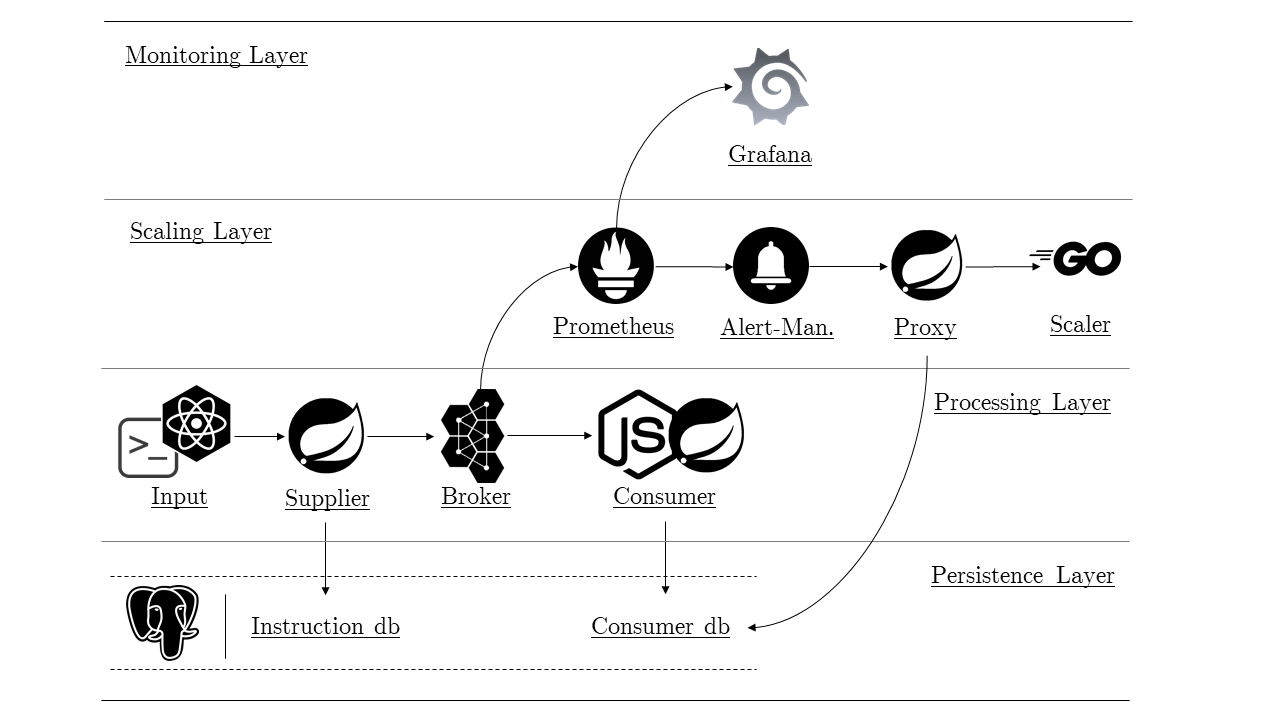
\includegraphics[width=\linewidth]{kapitel/problemloesung/implementierung/_img/overview-bw}
	\caption[Komponenten-Stack im Überblick]{Komponenten-Stack im Überblick}
	\label{fig:stackOverview}
\end{figure}

\begin{itemize}
  \item Persistenzschicht (engl. \emph{persistence layer}): Beinhaltet sämtliche Komponenten, die für das Abspeichern gegebener Datensätze in dazugehörige Datenbanken zuständig sind. Um Nebenläufigkeit zu ermöglichen, wird hier ebenfalls auf Schnittstellen über einen Message-Broker zurückgegriffen. Eine Manipulation der Daten findet auf dieser Ebene nicht statt.
  \item Verarbeitungsschicht (engl. \emph{processing layer}): Beinhaltet sämtliche Komponenten, die für die direkte Verarbeitung der Business-Logik zuständig sind. Die Kommunikation zwischen den Komponenten findet über eine REST-Schnittstelle sowie einen Message-Broker statt. Der Message-Broker stellt hierbei vor allem eine nebenläufige Verarbeitung der konsumierenden Komponenten sicher. Allerdings bietet dieser ebenfalls die Schnittstelle zur Skalierungsschicht (engl. \emph{scaling layer}).
  \item Skalierungsschicht (engl. \emph{scaling layer}): Beinhaltet sämtliche Komponenten zum Skalieren der konsumierenden Komponenten. Hierbei wird auf eine universelle Schnittstelle des Message Broker zurückgegriffen um entsprechende Metriken abzugreifen, die für die Evaluierung hinterlegter Regeln zur Skalierung verwendet werden. Ansonsten wird in Komponenten dieser Schicht das Zeitverhalten des Initialisierungsprozesses der konsumierenden Komponenten überwacht und an Schnittstellen der Persistenzschicht weitergeleitet.
  \item Monitoring Ebene: Diese Schicht besteht aus einer einzigen Komponente, deren Aufgabe es ist erhaltene Daten visuell darzustellen. Um einen zeitlichen Überblick zu geben, werden die Daten intern vom Werkzeug gespeichert. Da es sich um lokal verwaltete Datensätze handelt, die für den Rest der Applikation keinerlei Bedeutung darstellen, wurde darauf verzichtet eine Lösung zu finden, in der diese ebenfalls in einer Komponente der Persistenzschicht abgespeichert werden.
\end{itemize}

\newpage

\subsection{Komponenten im Überblick}
Es folgt eine kurze Zusammenfassung der Funktionalität sowie der Anforderungen an die jeweiligen Komponenten.

\subsubsection{Input}
Um es dem Benutzer zu ermöglichen, gezielte Messwerte zu erfassen, wird eine REST-Schnittstelle vom System bereitgestellt. Es ist zwar möglich, dass der Benutzer selbstständig Anfragen für diese Schnittstelle generiert und absendet, beabsichtigt ist allerdings, dass der Benutzer auf vordefinierte Skripte oder eine entsprechende Benutzeroberfläche zurückgreift. Die Benutzeroberfläche ist sehr funktional gehalten, sodass es zwar möglich ist, hierüber Anfragen an das System zu stellen, dennoch empfiehlt sich gerade für komplexere Anfrageszenarien der Gebrauch der bereitgestellten Bash-Skripte. Bezüglich der Skripte gibt es ebenfalls diverse Abstraktionsschichten. So ist es zum Beispiel möglich, mithilfe einer definierten Grammatik Anforderungen zu definieren, die sich beliebig kombinieren lassen. Hierzu wurden mehrere vordefinierte Dateien angelegt, deren Inhalt über ein entsprechendes Skript an das Backend geschickt werden kann. Allerdings gibt es weitere Skripte, die auf diesem Prozess aufsetzen und somit eine Abstraktionsschicht aufbauen, sodass sich der Endbenutzer hiermit nicht auseinandersetzen muss (detaillierte Beschreibung siehe Abschnitt \ref{ss:Input} \nameref{ss:Input}).

\subsubsection{Supplier}
Diese Komponente ist in der Lage, die vereinfachten Anfragen des Benutzers zu interpretieren und in Nachrichten umzuwandeln, die vom System verarbeitet werden können. Hierbei werden bereits an dieser Stelle der Verarbeitungspipeline diverse Informationen an die ursprüngliche Nachricht angeheftet, um im späteren Verlauf entsprechende Metriken zu berechnen. Außerdem erfolgt eine erste Kommunikation mit der Persistenzschicht, in der die übersetzten Benutzeranfragen abgespeichert werden. Hierbei wird direkt auf die Datenbank zugegriffen, da im System lediglich eine Singleton-Instanz des \emph{Suppliers} vorhanden ist. Zwar unterstützt die verwendete Postgres-Datenbank mehrere Klienten zur gleichen Zeit, nativ ist diese Anzahl jedoch begrenzt und muss angemessen konfiguriert werden. Des Weiteren stellt die Supplier-Komponente zwei Modi hinsichtlich der Geschwindigkeit bereit, in der Nachrichten an den Broker übermittelt werden. So ist es zum Beispiel möglich, Nachrichten über einen gewissen Zeitraum hinweg abzuschicken oder aber eine Transaktion zu bilden, in der alle auf einmal geschickt werden.

\subsubsection{Broker}
\label{ss:broker}
Ein Message-Broker stellt die Funktionalität bereit, Nachrichten über ein gegebenes Protokoll an mehrere Konsumenten zu vermitteln. Hierzu wurde eine Implementierung von Apache namens "\emph{Active MQ\footnote{\url{https://github.com/apache/activemq}}}" gewählt. Diese besitzt zwei Betriebsmodi, einmal das Arbeiten mit einer \emph{Topic} sowie mit einer \emph{Queue}. Eine Topic stellt ein \emph{Publisher-Subscriber-Muster} bereit, in dem alle eingehenden Nachrichten an alle registrierten Konsumenten verschickt werden \cite[Seite~33 ff.]{activemq-snyder}. Demgegenüber steht eine \emph{Queue} (Warteschlange), die eingehende Nachrichten lediglich an einen einzelnen Konsumenten übermittelt, wobei der Broker hierbei als eine Art Load Balancer\footnote{Erklärung \emph{Load Balancer} siehe Abschnitt \ref{sec:loadbalancer} \nameref{sec:loadbalancer}} agiert. In dem Prototypen wurde hierbei stets auf Warteschlangen zurückgegriffen, da eingehende Nachrichten stets von einer einzelnen Komponenteninstanz beantwortet werden. Bevor die Nachrichten jedoch aus einer der beiden Datenstrukturen entfernt werden, muss der betreffende Konsument eine \emph{Acknowledgement-Nachricht} an den Broker schicken, um zu signalisieren, dass die Nachricht nicht nur angenommen, sondern auch korrekt verarbeitet werden konnte. Je nach Empfangskomponente wird dieses Acknowledgement direkt von der verwendeten Library geschickt oder aber im Programmcode selbst explizit gesetzt. Es gilt weiterhin noch hervorzuheben, dass die eingeschriebenen Konsumenten bei neuen Nachrichten stets benachrichtigt werden und es clientseitig keine Logik braucht, um zum Beispiel event- oder intervallbasiert eine Abfrage an den Broker zu steuern. Da diese Komponente ebenfalls den Einstiegspunkt für das Monitoring-System \emph{Prometheus} (siehe Abschnitt \ref{ss:prometheus} \nameref{ss:prometheus}) darstellt, benötigt der Broker eine Schnittstelle über die er diesem Tool Messdaten zur Verfügung stellen kann. Die von ActiveMq bereitgestellt Schnittstelle nennt sich "\emph{Java Management Extension API (JMX)}" und ist die Standard-API zur Verwaltung von Java-Applikationen \cite[Seite~331 ff.]{activemq-snyder}.


\subsubsection{Consumer}
Die konsumierenden Komponenten empfangen die generierten Nachrichten und können beliebig skaliert werden. Sie implementieren die in Abschnitt \ref{ss:fiktiverWorkflow} definierten Arbeitsschritte. Hierbei wird auf diverse Bibliotheken zurückgegriffen, wobei die restliche Logik einfach gehalten wurde. Die Komponenten kommunizieren lediglich über eine Warteschlange des Message-Brokers mit dem Nachrichten-Supplier und über eine weitere mit der Persistenzschicht um die extrahierten Elemente abzulegen.


\subsubsection{Prometheus}
\label{ss:prometheus}
"\emph{Prometheus is an open source systems monitoring and alerting toolkit}" \cite[Seite~400]{oreillyPrometheus}. Es ist möglich über eine definierte Anfragensprache Daten Dritter zu verarbeiten. Diese Daten können über ein einfaches Textformat von den Komponenten ausgegeben werden. Es ist möglich dieses Textformat händisch zu schreiben, allerdings wird in der Praxis vermehrt auf Bibliotheken, die auf den Client zugeschnitten wurden, gesetzt. Prometheus ist unter der Apache 2.0 Lizenz veröffentlicht\footnote{https://github.com/prometheus/prometheus}, und wurde primär in der Programmiersprache Go implementiert. Das intervallbasierte Anfragen (engl. "\emph{scrapen}") der Metriken wird von der Prometheus-Komponente selbst durchgeführt, die zu überwachenden Komponenten müssen sich selbst nicht darum kümmern, Daten an Prometheus zu übermitteln. Im Prototypen werden hierbei mehrere Warteschlangen überwacht. Diese Warteschlangen bilden die Grundlage zur Visualisierung sowie zur Überwachung der nötigen Skalierungsschritte.


\begin{figure}[ht!]
	\centering
	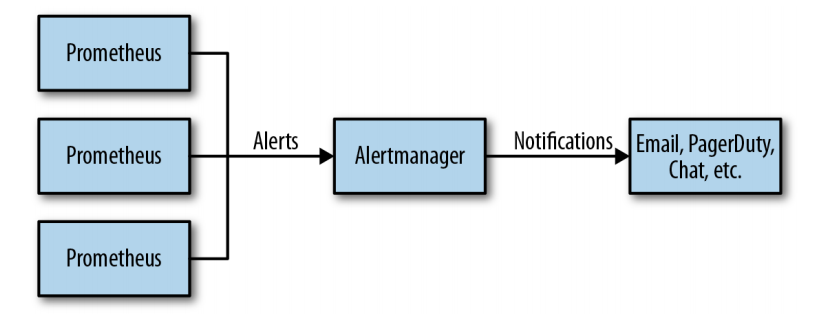
\includegraphics[width=.8\linewidth]{kapitel/problemloesung/implementierung/_img/alert-man-p291}
	\caption[Alert Manager - Übersicht]{Alert Manager - Übersicht \cite[Seite~291]{oreillyPrometheus}}
	\label{fig:alertManOverview}
\end{figure}

\subsubsection{Alert Manager}
"\emph{Alerting is one of the components of monitoring, allowing you to notify a human when there is a problem}" \cite[Seite~291]{oreillyPrometheus}. Prometheus bietet hierbei die Möglichkeit mithilfe der funktionalen Anfragesprache \emph{PromQl} diverse Bedingungen zu definieren unter denen dies geschehen soll. Da es in einer produktiven Containerumgebung durchaus möglich ist, dass mehrere Prometheus-Instanzen parallel arbeiten, wurde das Benachrichtigen in eine weitere Komponente (den \emph{Alert Manger}) ausgelagert. Dieser synchronisiert, sammelt und gruppiert die Alerts der verschiedenen Prometheus-Instanzen und sendet Benachrichtigungen an definierte Nachrichtenkanäle, die sich beispielsweise aus einem Emailpostfach, einer Pagernachricht oder Chatnachricht auf Plattformen wie Slack zusammensetzen können (siehe Abbildung \ref{fig:alertManOverview} \nameref{fig:alertManOverview}). Im Prototypen wurden die eingehenden Alerts derartig übersetzt, dass sie von der Proxy-Komponente interpretiert werden können.


\subsubsection{Scaler Proxy}
Diese Komponente bietet eine REST-Schnittstelle, die im Alert-Manager hinterlegt wird. Sobald eine der Regeln anschlägt, wird der Aufruf an diese Komponente weitergeleitet. Im Endeffekt dient diese Komponente lediglich als Proxy-Service, da ihre primäre Aufgabe darin besteht diese Nachricht an eine weitere Komponente weiterzuleiten. In einer produktiven Umgebung würde diese Komponente komplett enfallen, da es möglich ist den Alert-Manager derartig zu konfigurieren, dass er direkt die öffentlichen Schnittstellen der Scaler-API anspricht. Es wurde sich dennoch für das Zwischenschalten eines solchen Proxy-Services entschieden um genauere Messwerte zu erhalten. Gerade hinsichtlich der Initialisierungsphasen von Containern ist es angebracht so kurz vorher wie möglich einen Timestamp zu setzen. Da es keine Möglichkeit gibt direkt in die Konfiguration der Scaler-API einzugreifen ist diese Lösung der nächstbeste Ansatz. Sobald eine Skalierungsanfrage weitergeleitet wurde, wird diese noch unbeantwortete Anfrage intern in einer Datenstruktur abgelegt. Sobald ein entsprechender Container komplett initialisiert wurde, ruft dieser eine weitere Schnittstelle des Proxy-Services auf. Daraufhin wird ein \emph{Acknowledgement-Timestamp} in der hinterlegten Anfrage gesetzt und an die Persistenzschicht weitergeleitet. 

Außerdem bietet diese Komponente die Möglichkeit für den Benutzer, direkt Exemplare eines Consumers hochzufahren. Die verwendete Schnittstelle dient sowohl als Umgehung des herkömmlichen Programmflusses als auch zur Generierung der Metrikberechnung, ohne auf den nachrichtenbasierten Skalierungsalgorithmus zurückgreifen zu müssen (siehe Abschnitt \ref{par:specContainer} \nameref{par:specContainer}). Über dedizierte Endpunkte können diese Metriken als .csv Datei ausgelesen werden. 


\subsubsection{Scaler}
"\emph{The goal of the Docker Scaler project is to provide a REST HTTP interface to scale services and nodes}" \cite{docker-scaler}. Außerdem werden mit jeder Skalierungsanfrage Statusinformationen über die aktuelle sowie zukünftige Anzahl von Instanzen des zu skalierenden Services zurückgegeben, die es dem Proxy-Service ermöglichen, davon ausgehend einen Skalierungsstop für neue Anfragen beizubehalten oder aufzuheben. Dieser ist nötig, damit das System keine weiteren Skalierungsprozesse startet, wenn bereits aktive Skalierungen vorgenommen werden. Im Prototypen wurde diese Komponente mit minimaler Konfiguration direkt in den Stack übernommen.


\subsubsection{Grafana}
Wenn es zum Alert durch den Alert Manager kommt, wird in einer Produktivumgebung der erste Schritt sein die Performanz des Systems durch dedizierte Dashboards zu überprüfen \cite[Seite~97]{oreillyPrometheus}. Grafana ist ein Werkzeug, das dies über eine Weboberfläche direkt im Browser ermöglicht. Es bietet die Möglichkeit Graphen, Tabellen und weitere Visualisierungskomponenten zu erstellen um zum Beispiel die Latenzzeit oder CPU-Auslastung zu überprüfen. Diese Metriken können für das ganze System oder nur einen Teil generiert werden. Es ist das bevorzugte Visualisierungswerkzeug für Prometheus, bietet allerdings ebenfalls Unterstützung für verschiedene weitere Systeme wie zum Beispiel \emph{Graphite}, \emph{Elasticsearch} oder \emph{PostgreSQL}. Im Prototypen wurden hierbei sämtliche Metriken der Warteschlangen, sowie sonstiger überwachter Komponenten, grafisch aufbereitet. Hierbei ist auch ein zeitlicher Ablauf zu erkennen.


\subsubsection{Mock scaler api}
Diese Komponente ist nicht Kernbestandteil des Komponenten-Stacks. Sie dient lediglich während der Entwicklungszeit dazu, die Scaler-API zu emulieren. So ist es zum Beispiel möglich lokal eine Instanz des Scaler-Proxy Projekts in einer beliebigen IDE als Standard Spring Projekt auszuführen. Sämtliche Skalierungs-Anfragen können von dieser Komponente angenommen werden, da sie auf dem gleichen Port wie der "\emph{echte}" Scaler läuft, wobei sie dabei ebenfalls in der Lage ist diverse Rückgabenachrichten an den Klienten zu übergeben.


\subsection{Input}
\label{ss:Input}

Der Benutzer besitzt die Möglichkeit, sowohl über eine Benutzeroberfläche als auch über Bash-Skripte Benchmark-Anfragen an das System zu stellen. Im Folgenden wird beides im Detail erläutert.

\label{ss:bash}
\subsubsection{Aufbau}
In der folgenden Abbildung ist der Aufbau des Bash-Projektes dargestellt. Der Benutzer besitzt drei Möglichkeiten, Anfragen an das System zu stellen. Für jeden Einstiegspunkt wurde ein entsprechendes Bash-Skript zur Verfügung gestellt.

\begin{figure}[ht!]
	\centering
	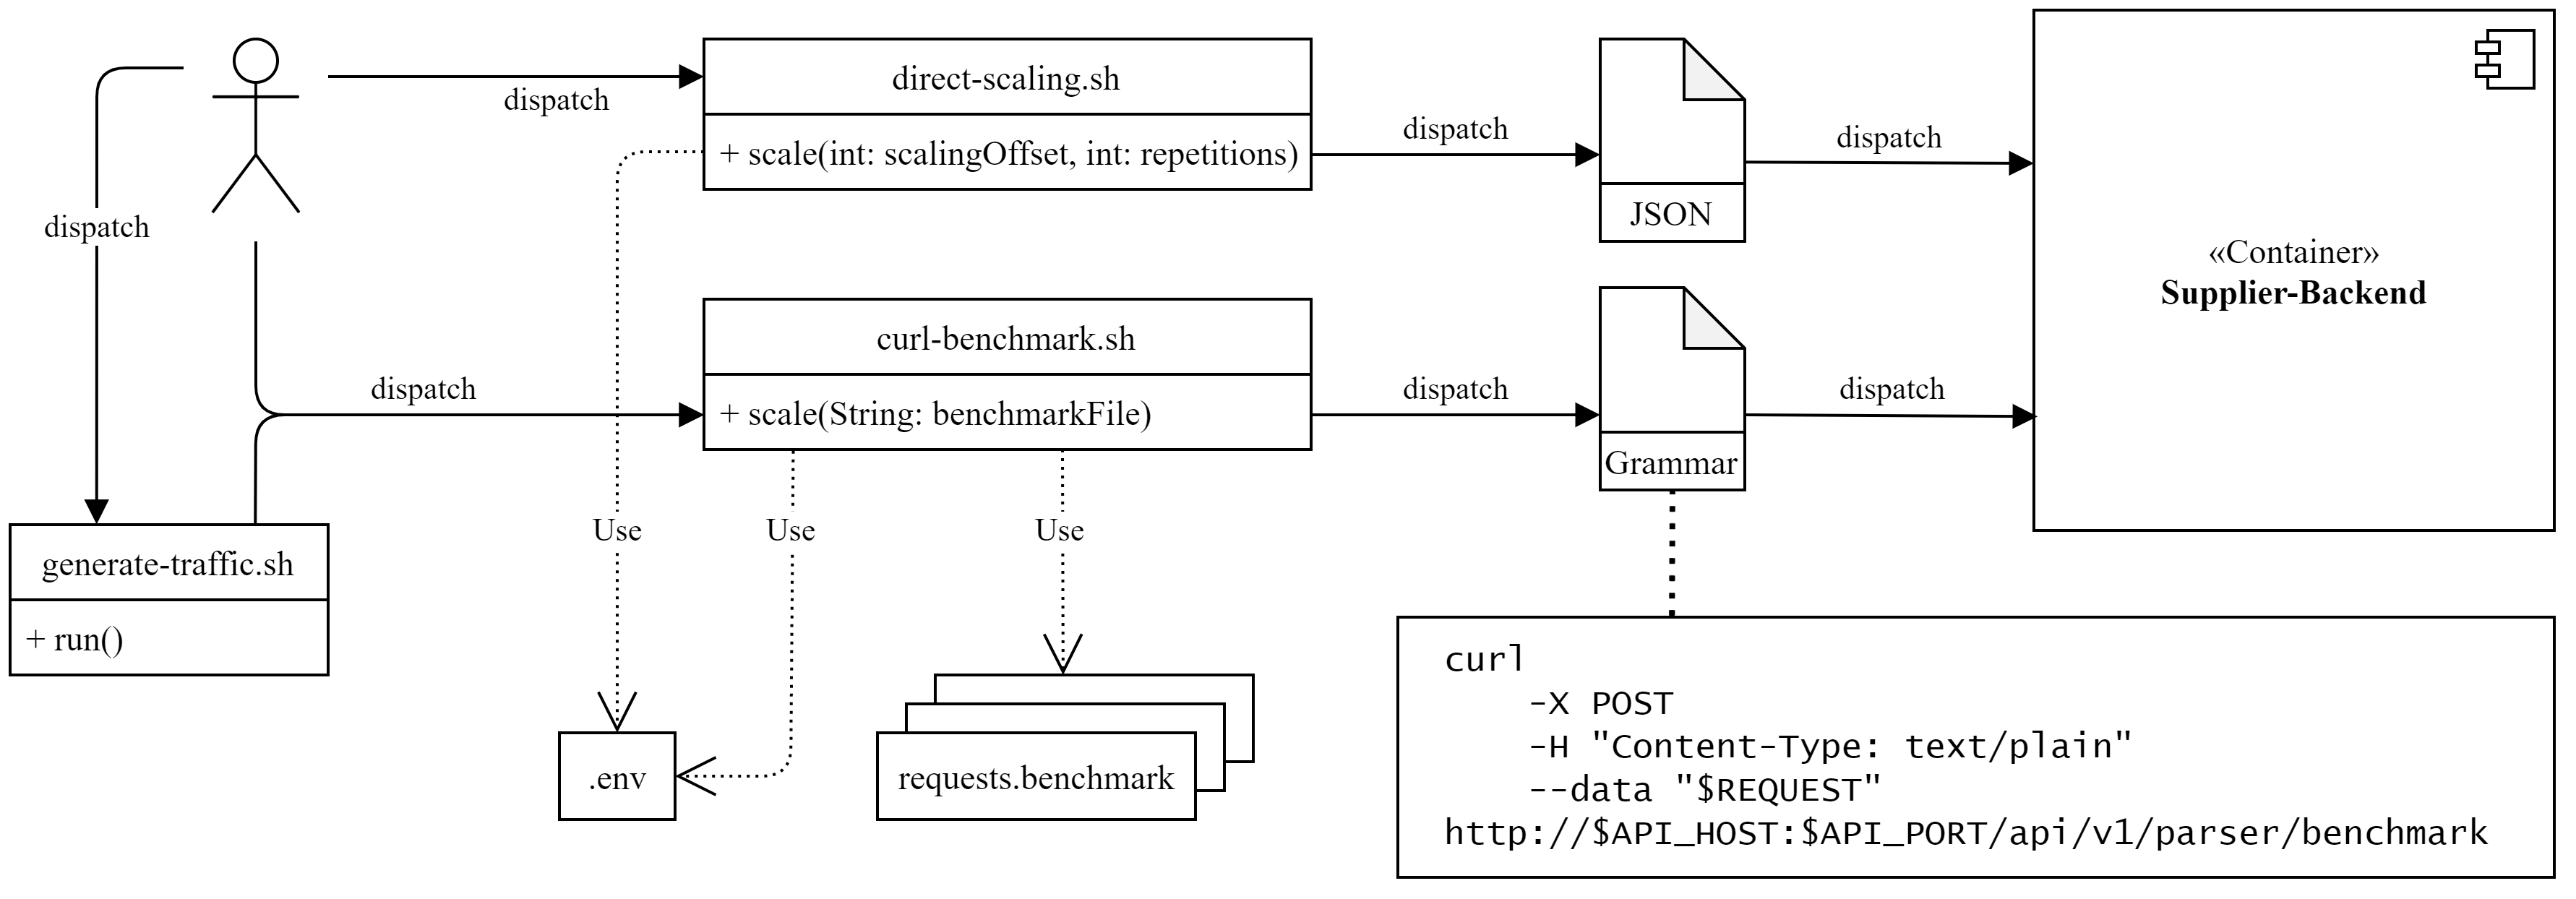
\includegraphics[width=\linewidth]{kapitel/problemloesung/implementierung/_img/input-uml}
	\caption[Bash Input UML]{Bash Input UML}
	\label{fig:bashOverview}
\end{figure}

\begin{itemize}
  \item \emph{direct-scaling.sh}: Bietet die Möglichkeit eine direkte Skalierungsanfrage an das System zu senden, ohne Payment-Messages verwenden zu müssen. Als Parameter werden die Skalierungsanzahl sowie die Wiederholungen erwartet (genauere Erklärung siehe \ref{erklaerungDirScal} \nameref{erklaerungDirScal}).
  \item \emph{curl-benchmark.sh}: Sendet eine Skalierungsanfrage mit dem Inhalt einer Datei, dessen Pfad als Eingabeparameter verarbeitet wird. Die Datei besitzt die Dateiendung \emph{.benchmark}, wobei der Inhalt einer spezifizierten Grammatik folgt (siehe \ref{lst:instruction-grammar} \nameref{lst:instruction-grammar}).
  \item \emph{generate-traffic.sh}: Dient als vereinfachter Einstiegspunkt für den Benutzer. Hierbei werden rekursiv alle verfügbaren \emph{.benchmark} Dateien des Verzeichnisses der Reihe nach dem \emph{curl-benchmark} Skript übergeben.
\end{itemize}

Im folgenden Listing (siehe Listing \ref{verb:scriptStruct} \nameref{verb:scriptStruct}) ist ein Auszug der Projekt-Struktur abgebildet. Neben den genannten Skripten sind sämtliche \emph{.benchmark} Dateien nach Services in Unterordner aufgeteilt worden. Die \emph{.env} Datei beinhaltet die Verbindungsdaten zum Komponenten-Stack. Diese müssen bei der ersten Ausführung vom Benutzer angeglichen werden. Im Wesentlichen beschränkt sich dies auf die IP-Adresse des Systems, falls der Benutzer in der Stack-Konfiguration entsprechende Änderungen vornimmt, sind diese an dieser Stelle ebenfalls zu vermerken.

\label{verb:scriptStruct}
\begin{minipage}{\linewidth}
\begin{lstlisting}[caption={Bash Skript - Struktur},style=bashStyle]
  $ tree request-scripts/ -a -L 3 --charset=ascii
  request-scripts/
  |-- curl-benchmark.sh
  |-- direct-scaling.sh
  |-- .env
  |-- generate-traffic.sh
  |-- README.md
  `-- requests
      |-- mixed
      |   |-- benchmark_large_mixed.benchmark
      |   |-- benchmark_medium_mixed.benchmark
      |   `-- benchmark_small_mixed.benchmark
      ...
\end{lstlisting}
\end{minipage}

\subsubsection{Manuelles Skalieren}
\label{erklaerungDirScal}
Hierfür wird auf ein Bash-Skript namens "\emph{direct-scaling}" zurückgegriffen. Das Skript nimmt zwei Parameter entgegen. Der Erste beschreibt die Anzahl der Instanzen, zu der das System skaliert werden soll, wobei hierbei eine inkrementelle Erhöhung von einer Instanz pro Durchlauf durchgeführt wird. Der zweite Parameter gibt die Wiederholungen dieser testweisen Skalierung an. Der Aufruf \verb+./direct-scaling.sh 10 20+ resultiert beispielsweise darin, dass sowohl für den Node.js- als auch Spring-Boot-Service jeweils 10 Skalierungsschritte durchgeführt werden. Wenn zum Beispiel bereits ein Node.js-Container läuft, wird im ersten Test eine weitere Instanz angefordert. Sobald die beiden Instanzen verfügbar sind, wird der Alert-Manager durch die Prometheus-Komponente angewiesen die überflüssige Instanz zu löschen. Sobald wieder ein einziger Container läuft, wird dieser Schritt neunzehn weitere Male wiederholt. Anschließend erfolgt die nächste Skalierung bei der nun zwei neue Container kreiert werden sollen, anstatt wie vorher nur ein weiterer. Auch hier folgen 20 Wiederholungen. Diese Schritte werden solange durchgeführt bis zehn Container zwanzig Mal instanziiert wurden.

\label{lst:direct-scaling}
\begin{minipage}{\linewidth}
\begin{lstlisting}[caption={direct-scaling.sh},style=bashStyle]
...

request() {
  curl "http://$HOST:$DIRECT_SCALING_PORT/manual-scale?additionalCnt=$1&service=$4"
}

node_request() {request $1 $2 $3 'NODE'}
spring_request() {request $1 $2 $3 'SPRING'}

for scalingOffset in $(seq 1 $1)
do 
  for curr_rep in $(seq 1 $2)
	do 
    node_request $scalingOffset $curr_rep $2
    spring_request $scalingOffset $curr_rep $2
  done
done
\end{lstlisting}
\end{minipage}

\subsubsection{Skalieren mithilfe einer Grammatik}
Das beschriebene Skript sowie der zugrunde liegende Http-Endpunkt bieten eine Möglichkeit, das Skalieren als Reaktion auf unbeantwortete Nachrichten zu umgehen. Um jedoch einen herkömmlichen Testdurchlauf zu starten, greift der Benutzer auf einen Endpunkt vom \emph{Supplier} zurück: 

\begin{verbatim}
  curl 
    -X POST 
    -H "Content-Type: text/plain" 
    --data "$REQUEST" 
    "http://$API_HOST:$API_PORT/api/v1/parser/benchmark"
\end{verbatim}

Es handelt sich hierbei um eine POST-Anfrage. Im Body wird der Dateiinhalt eines für diesen Zweck verfassten Skripts angeheftet. Im Projekt wurden diverse Beispiele verfasst. Diese liegen im Ordner \emph{./requests} und tragen die Dateiendung "\emph{.benchmark}". Der Inhalt korrespondiert zu einer spezifizierten Grammatik (siehe Listing \ref{lst:instruction-grammar} \nameref{lst:instruction-grammar}).

\label{lst:instruction-grammar}
\begin{verbatim}
  request     := batch*
  batch       := serviceName { instruction | instruction,* };
  serviceName := SPRING | NODE
  instruction := BENCHMARK ( messageCnt, duration ) | WAIT ( duration )
  messageCnt  := [0-9]+
  duration    := [0-9]+
\end{verbatim}

Es können beliebig viele Batchanfragen an dem Anfragenbody angeheftet werden. Eine Batchanfrage stellt in diesem Zusammenhang eine Gruppe von Skalierungsanfragen an einen bestimmten Service dar, wobei diese mindestens eine Skalierungsinstruktion enthalten müssen. In diesem System gibt es zwei wesentliche Skalierungsinstruktionen: 

\begin{enumerate}
  \item BENCHMARK: Nimmt zwei Parameter entgegen. Der erste spezifiziert, wie viele neue Instanzen erstellt werden sollen, während der Zweite angibt, über welchen Zeitraum dies geschehen soll. Alle numerischen Angaben müssen einen positiven Ganzzahlwert enthalten. Da das System selbstständig in der Lage sein soll diese Instanzen wiederum auf ein gesetztes Minimum zu reduzieren, wurde sich aktiv dagegen entschieden, das Herunterskalieren in die Grammatik aufzunehmen, um dem Benutzer eine möglichst einfach gehaltene Schnittstelle zur Verfügung zu stellen.
  \item WAIT: Diese Instruktion erwartet lediglich einen einzigen Parameter, der angibt wie viele Millisekunden gewartet werden soll, bevor die nächste Instruktion dem System übergeben wird. 
\end{enumerate}


Damit der Benutzer allerdings direkt Anfragen ausführen kann, ohne sich mit der Grammatik beschäftigen zu müssen, wurde ein weiterer Skript-Aufsatz 
für das \emph{curl-benchmark} Skript entwickelt. Dieses trägt den Namen "\emph{generate-traffic.sh}" und sucht rekursiv absteigend in der eigenen Directory nach Dateien mit der entsprechenden Endung. Anschließend werden diese Skripte an das \emph{curl-benchmark} der Reihe nach als Parameter übergeben.

\subsubsection{Benutzeroberfläche}
Im Rahmen dieser Thesis wurde die Benutzeroberfläche mithilfe des Javascript-Frameworks \emph{React.js} entwickelt. Es ist möglich über diverse Select-Felder die voreingestellten Pfaden, sowie Payment Optionen auszuwählen. Außerdem ist es möglich, die Anzahl sowie die Zeitspanne der Anfrage zu spezifizieren. Beim Initialisierungsprozess dieses Projekts starten zuallererst alle dargestellten React-Komponenten. React.js ist ein komponentenbasiertes Framework, hierbei werden sämtliche visuellen Elemente als einzelne Komponenten betrachtet, wobei es möglich ist, diese Komponenten zu gruppieren und somit neue Komponenten zu formen. Außerdem ermöglicht das Framework diesen Komponenten einen sogenannten \emph{State} anzuheften, in dem Daten hinterlegt werden können. Wenn diese an irgendeiner Stelle modifiziert werden, erkennt React dies und rendert die betroffene Komponente sowie alle untergeordneten Komponenten neu. Dies ist insbesondere hilfreich um die Formulareinträge direkt abzuspeichern. Bei der Initialisierung versucht die Frontend-Komponente die darzustellenden Optionen vom \emph{Supplier} zu fetchen. Dieser beantwortet diese Anfrage mit den Daten, die im Anschluss in der Oberfläche angezeigt werden. Wenn der Benutzer darauf folgend Daten auswählt beziehungsweise Daten in die Felder einträgt, werden hierfür zugeschnittene Eventhandler-Funktionen ausgelöst. Diese Eventhander registrieren die Datenauswahl und speichern sie direkt im State der Komponente ab. Wenn der Benutzer nun auf den Button zum Absenden der Anfrage klickt, muss hierbei lediglich der State ausgelesen werden und an die entsprechende Backend-API-Schnittstelle geschickt werden. In Abbildung \ref{fig:reactUi} \nameref{fig:reactUi} wurde hierfür der aktuelle Stand der Oberfläche dargestellt.

\begin{figure}[ht!]
	\centering
	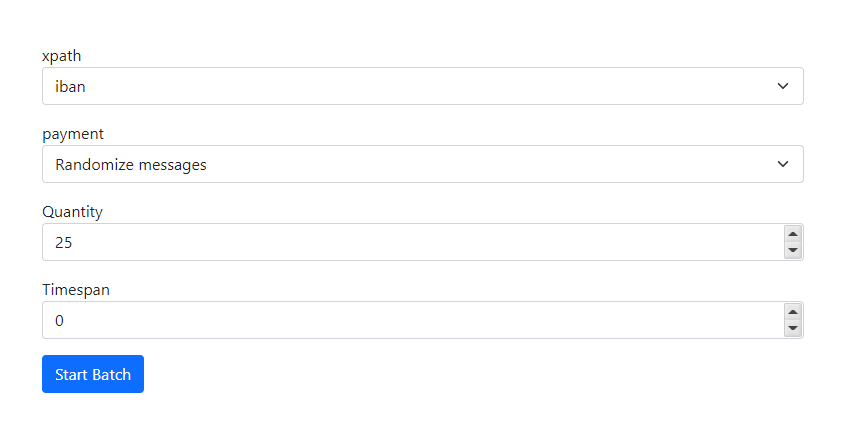
\includegraphics[width=.9\linewidth]{kapitel/problemloesung/implementierung/_img/react01}
	\caption[React - Benutzeroberfläche]{React - Benutzeroberfläche}
	\label{fig:reactUi}
\end{figure}

Während der Entwicklungszeit des restlichen Systems wurde das Arbeiten mit der Benutzeroberfläche allerdings vermehrt zum Flaschenhals. Sobald ein neues Feature oder ein neuer Datensatz in eine Anfrage integriert wurde oder sich das zugrunde liegende Datenmodell änderte, war es jedes Mal ein großer Aufwand dies ebenfalls in der Oberfläche anzupassen. Da die vorher spezifizierte Grammatik sowie die zugrunde liegende API einen deutlich flexibleren Ansatz und eine komplexere Ablauflogik ermöglichen wurde sich bereits früh in der Entwicklung entschlossen diesen Ansatz der grafischen Benutzerführung nicht weiterzuverfolgen. Die Oberfläche dient hierbei eher als ein \emph{Proof of concept}, um darzustellen, wie ein solches Projekt konfiguriert werden muss. Da dem skriptbasierten Ansatz dieselben API-Schnittstellen zugrunde liegen wie dem oberflächenbasierten Ansatz, ist es ohne Probleme möglich das aktuelle React-Projekt den überarbeiteten Gegebenheiten anzupassen, falls dies in Zukunft gewünscht sein sollte.


\subsection{Supplier Backend}
Bei dieser Komponente handelt es sich um ein Spring Projekt, dessen Aufgabe es ist, Benutzeranfragen in Nachrichten zu übersetzen, die vom System interpretiert und verarbeitet werden können. Die Schnittstelle für den Benutzer besteht hierbei aus einer REST-API, die über Tools wie zum Beispiel curl angesprochen werden kann.

\subsubsection{Generelle Spring Projektübersicht}
\label{ss:springProj}
Da diese Komponente bezüglich der Struktur eines Spring-Projekts alle wesentlichen Merkmale besitzt, wird die genutzte Projektstruktur an dieser Stelle etwas näher erläutert. 

Das Muster, nach dem sämtliche Komponenten des Komponenten-Stacks entwickelt wurden, wird als \emph{Layered Architecture Pattern} oder \emph{n-tier pattern} bezeichnet \cite{oreilly-layered-arch}. Es stellt einen weitverbreiteten Standard in Java Enterprise Applikationen dar und zeichnet sich durch die klare Unterteilung der verschiedenen Hierarchien aus (siehe Abbildung \ref{fig:layeredArchitecture}). Sämtliche Packages innerhalb der Spring-Projekte finden sich innerhalb einer der Schichten wieder. Es sei ebenfalls hervorzuheben, dass sämtliche Schichten stets nur mit ihren direkt angrenzenden Schichten kommunizieren. Dies stellt ein übersichtliches Design sicher.
\newpage

\label{verb:supplierStruct}
\begin{lstlisting}[caption={Supplier Backend - Struktur},style=bashStyle]
  $ tree stack/supplier-backend/ -a -L 7 --charset=ascii
  stack/supplier-backend/
  |-- Dockerfile
  |-- pom.xml
  `-- src
      `-- main
          |-- java
          |   `-- dps
          |       `-- hoffmann
          |           `-- producer
          |               |-- config
          |               |-- controller
          |               |-- model
          |               |-- properties
          |               |-- repository
          |               |-- response
          |               |-- service
          |               `-- SupplierBackendApplication.java
          `-- resources
              |-- application-dev.properties
              |-- application-prod.properties
              `-- application.properties
\end{lstlisting}


\begin{figure}[ht!]
	\centering
	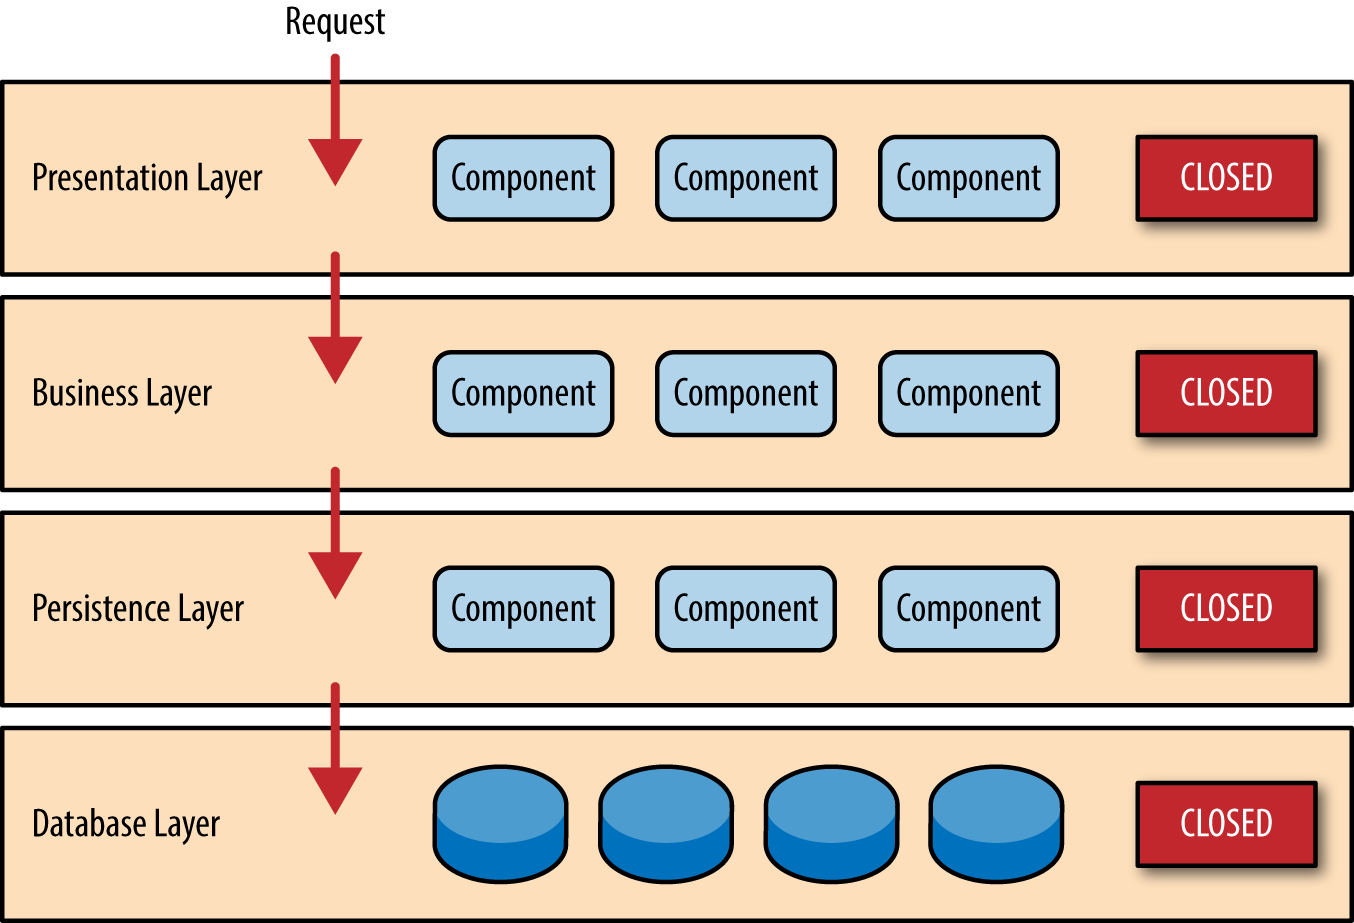
\includegraphics[width=.7\linewidth]{kapitel/problemloesung/implementierung/_img/dataflow-overview-01}
	\caption[Layered Architecture]{Layered Architecture \cite{oreilly-layered-arch}}
	\label{fig:layeredArchitecture}
\end{figure}


\begin{itemize}
  \item \emph{controller}: Dieses Package stellt alle Klassen bereit, welche direkt vom Benutzer angesprochen werden. Typischerweise handelt es sich zumindest im implementierten Stack um REST-Schnittstellen, aber auch andere Typen (Soap, etc.) bieten entsprechende Implementierung an. Klassen dieses Packages werden allgemeinhin als Controller bezeichnet und bilden eine erste Interaktionsschicht, welche keinerlei Business-Logik enthält. Bei diesem Package handelt es sich um einen Teil des Presentation-Layers. Die Daten werden angenommen aber nicht direkt verarbeitet. Dies geschieht in sogenannten Services, die spezifische Funktionalität implementieren. Controller dienen hierbei als Verteiler der eingehenden Nachrichten an diese Services. Die Service-Instanzen werden den Controllern über den Spring-Context mittels Dependency Injection\footnote{Dependency Injection: Verwendung von Objektinstanzen, welche durch einen IoC Container verwaltet werden.} bereitgestellt, sodass sich der Entwickler selbst nicht mit der Instanziierung etc. zu beschäftigen braucht. 

  \item \emph{service}: Dieses Package enthält ausschließlich Service-Implementierungen. Ein Service stellt einen logischen Funktionsbaustein der Anwendung dar und kann über den Spring-Context bereitgestellt werden. Services werden dem \emph{Business Layer} des Schichtenmodells zugeordnet.

  \item \emph{repository}: Spring bietet über entsprechende Dependency-Starter-Konfigurationen die JPA-Implementierung \emph{Hibernate} als nativen Support für die Anbindung an eine Datenbank. Dieses Package enthält Interfaces welche die Treiberschnittstelle beerben. Mithilfe spezifizierter Namenskonventionen ist es möglich Methodensignaturen für Datenbankanfragen zu gestalten. Das Framework generiert hieraus die entsprechenden SQL-Abfragen. Klassen dieses Packages lassen sich dem \emph{Persistence Layer} des Modells zuordnen.

  \item \emph{config}: Klassen dieses Packages instanziieren, beziehungsweise konfigurieren Spring-Beans. Es gibt bei vielen voreingestellten Spring-Komponenten die Möglichkeit Beans über Annotations in der implementierenden Klasse zu erzeugen. In bestimmten Situationen wird jedoch Zugriff auf die Instanz selbst zum Initialisierungszeitpunkt gebraucht um entsprechende Konfigurationsschritte zu unternehmen. Dies geschieht standardmäßig in diesem Package. Da dieses Package lediglich eine unterstützende Funktion einnimmt, wird es im Schichtenmodell nicht direkt aufgeführt. Um jedoch eine übersichtliche Projektstruktur zu gewährleisten, werden diese Klassen nicht in Packages der zu konfigurierenden Komponenten mit eingefügt, sondern gesondert angelegt.

  \item \emph{model}: Klassen, welche lediglich zum Abbilden bestimmter Datensätze genutzt werden, residieren in diesem Package. Hierbei ist es irrelevant, ob es sich um JPA-Entitäten oder herkömmliche POJOs handelt. Da es sich bei der Funktionalität der Klassen dieses Packages ebenfalls um eine unterstützende Funktion handelt, wird es ebenfalls nicht direkt im Schichtenmodell aufgeführt.

  \item \emph{properties}: Spring bietet die Möglichkeit Daten aus den Konfigurationsdateien innerhalb der Resources direkt in den Application-Context zu laden. Diese Klassen bilden eine Unterkategorie der beschriebenen Konfigurationsklassen.
  
  \item \emph{utils}: Klassen, die lediglich mit Business-Logik gefüllt sind und nicht vom Spring-Container verwaltet werden, sondern direkt im Programmcode instanziiert oder aufgerufen werden, residieren in diesem Package. Bei der Funktionalität der Klassen dieses Packages handelt es sich in der Regel um statische Hilfsmethoden die von Instanzen des \emph{Business Layers} verwendet werden.
  
  \item \emph{resources}: Die genutzte Verbindungs-Konfiguration zwischen Komponenten des Stacks werden innerhalb der \emph{.properties} Dateien verwaltet. Es ist möglich auf diese Information über den Dependency-Injection-Mechanismus innerhalb der Klassen zuzugreifen. Die hierbei hinterlegten Daten können zum Buildzeitpunkt direkt in das Artifact eingebunden werden. Sie stehen zur Laufzeit zur Verfügung und stellen ähnlich wie die Klassen des \emph{model} packages lediglich relevante Daten dar, beinhalten allerdings keine zusätzliche Programmlogik. 

\end{itemize}

\newpage

\subsubsection{Programmfluss}
Im folgenden UML-Diagramm (siehe Abbildung \ref{fig:supplierUml}) wurden ein Teil der Klassen des Suppliers dargestellt. Es wurde sich hierbei auf die wesentlichen Logikbausteine konzentriert. 

\begin{figure}[ht!]
	\centering
	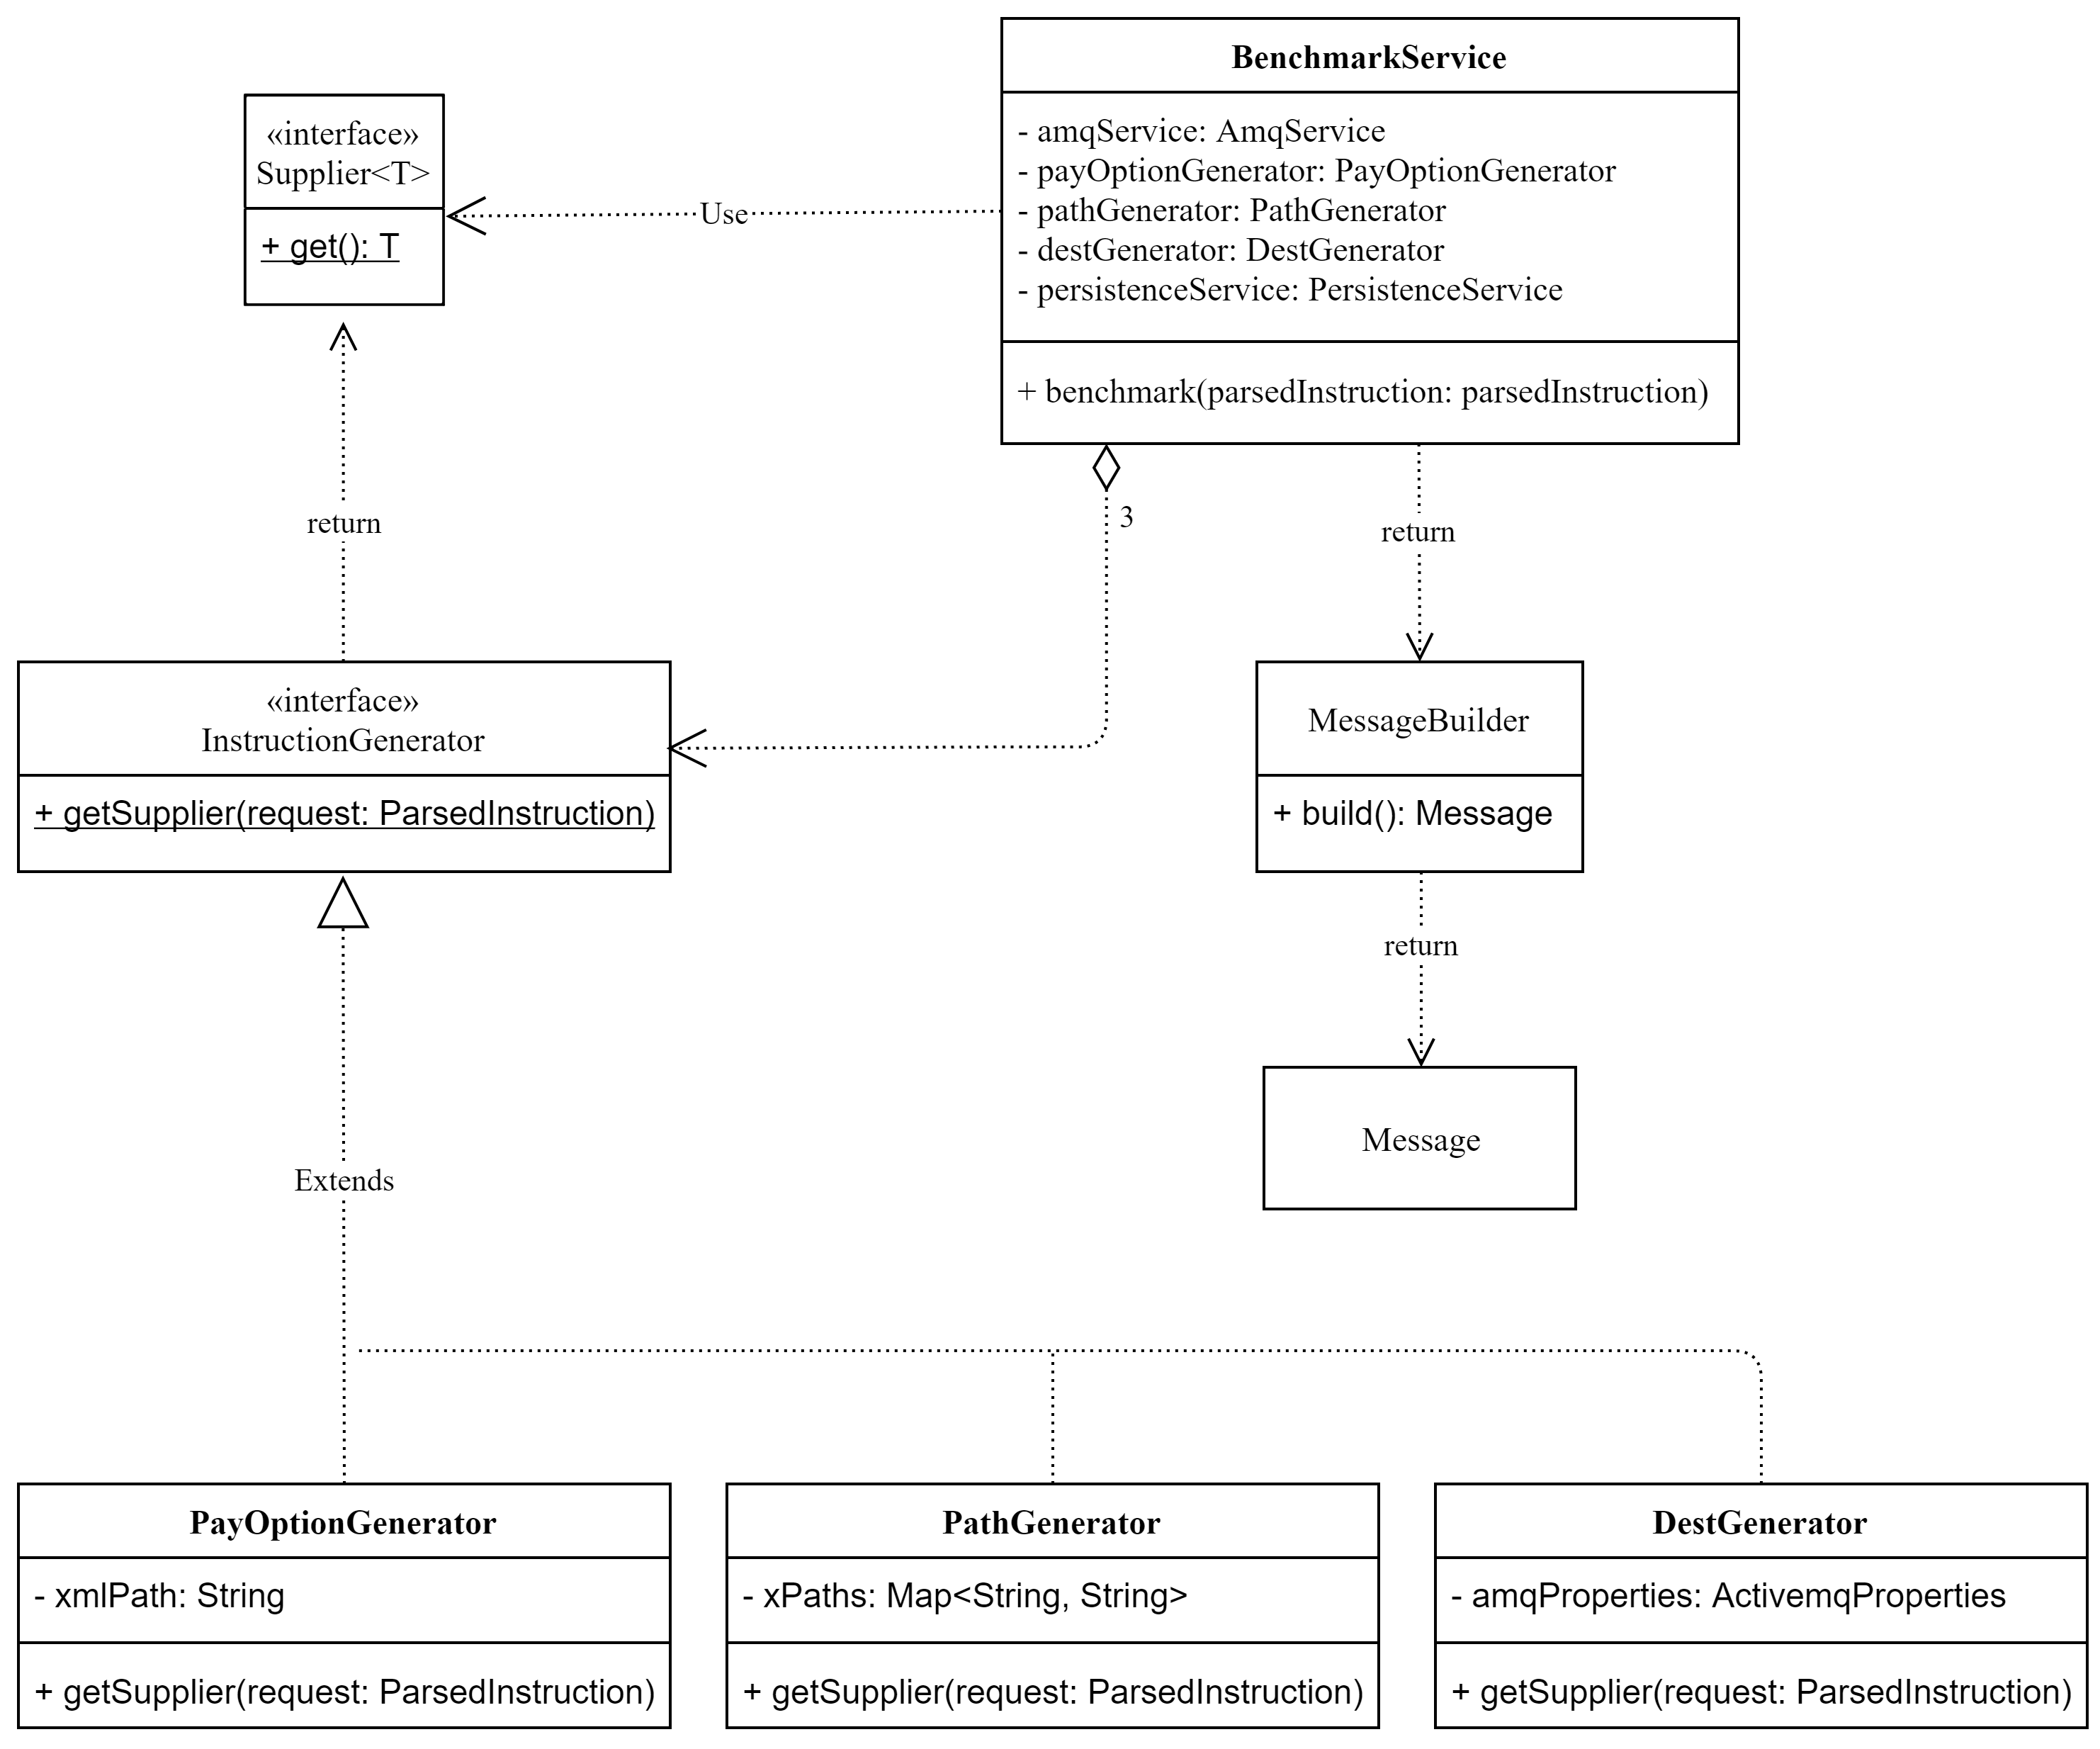
\includegraphics[width=\linewidth]{kapitel/problemloesung/implementierung/_img/supplier-uml}
	\caption[Backend Supplier UML]{Backend Supplier UML}
	\label{fig:supplierUml}
\end{figure}

Es gibt primär drei Einstiegspunkte für den Programmfluss. Der Benutzer möchte mithilfe der Benutzeroberfläche oder eines Curl-Aufrufs neue Nachrichten generieren, oder es wird auf die Dateiinhalte, die einer Grammatik folgen zurückgegriffen. Bei beiden Endpunkten wird im Controller eine Instanz vom Typ \emph{ParsedInstruction} erstellt. Diese enthält alle relevanten Informationen, die vom verarbeitenden \emph{BenchmarkService} gebraucht werden. Bei der API-Anfrage durch den Curl-Aufruf lässt sich das Instanziieren direkt über das Parsen vom empfangenen JSON umsetzen, während bei der Grammatik ein weiterer Service (\emph{RequestParserService}) verwendet wird, der aus der erhaltenen Grammatik diverse \emph{ParsedInstruction} Instanzen erstellt.

Wie im UML-Diagramm zu erkennen, werden aus der erhaltenen Instruktionsinstanz über verschiedene Generator-Implementierungen diverse Callbacks erstellt, die zum Absetzen der Nachrichten in das System genutzt werden. Ein Auszug des zugrunde liegenden Codes folgt in Listing \ref{lst:supplierServiceImpl} \nameref{lst:supplierServiceImpl};

\begin{minipage}{\linewidth}
\begin{lstlisting}[style=javaStyle,caption={Supplier - Service},label=lst:supplierServiceImpl]
  
      ...

      // create generator instances
      Supplier<String> xPathSupplier = pathGenerator.getSupplier(parsedInstruction);
      Supplier<String> paymentSupplier = payOptionGenerator.getSupplier(parsedInstruction);
      Supplier<String> destinationSupplier = destGenerator.getSupplier(parsedInstruction);
      BiConsumer<PaymentMessage, Supplier<String>> amqConsumer =
              amqService.getConsumer(sessionIsTransacted);

      ...

      for (int i = 0; i < parsedInstruction.getMessageCnt(); i++) {

          // use generator instances to dynamically create message
          PaymentMessage payment = PaymentMessage.builder()
                  .batchId(batchId)
                  .xPath(xPathSupplier.get())
                  .content(paymentSupplier.get())
                  .sentTimestamp(now())
                  .build();

          amqConsumer.accept(payment, destinationSupplier);

          Thread.sleep(durationMillis);
      }
  }

  ...
  
\end{lstlisting}
\end{minipage}

In dem beschriebenen Listing ist zu erkennen, wie diese Generatoren genutzt werden. Sie extrahieren aus der gegebenen Instruktionsinstanz die jeweils relevanten Werte für ihren Anwendungsfall (Zeile 5 -- 9) und können bei der Erstellung der Nachrichten als Callback verwendet werden, und dynamisch neue Werte erstellen (Zeile 16 -- 21). Hierbei wurde auf diese Callback-Struktur zurückgegriffen, da die gegebenen Werte in der Instruktion selbst als Instruktionen verstanden werden sollen.

\paragraph{Beispiel xPathSupplier} 
Der XPath gibt an, welches XML-Element bei der Verarbeitung durch den Consumer im Detail extrahiert werden soll (bspw. IBAN, Betrag etc.). Es ist jedoch auch möglich, dass der Benutzer bei der API-Anfrage hierbei keinen genauen XPath angibt sondern möchte, dass hierbei ein beliebiges Element extrahiert werden soll. Dazu wird der Wert "\emph{Randomize}" in die Instruktion eingetragen. Dies ist sinnvoll um etwas Variation in die spätere Verarbeitung zu bekommen um bessere Messwerte erzielen zu könnnen. Im System wurden hierfür beispielhaft einige XPath Pfade manuell hinterlegt. Der Supplier hat intern Zugriff auf diese Sammlung. Je nachdem ob ein spezifischer Wert ausgegeben werden oder dieser variieren soll, wird stets der selbe Wert oder aber unterschiedliche Werte ausgegeben. Ähnliches gilt für die anderen verfügbaren Generator-Instanzen.

\newpage

\subsection{Consumer-Komponente}

Im folgenden UML-Diagramm ist die grundlegende Klassenstruktur der beteiligten Logikbausteine des Spring-Konsumenten zu erkennen. Da das Node.js-Projekt einen sehr ähnlichen Aufbau besitzt, wird im Folgenden lediglich der Ablauf der Spring Komponente zusammengefasst. Sämtliche Informationen lassen sich jedoch nahtlos auf die Node.js-Umgebung übertragen. 

\begin{figure}[ht!]
	\centering
	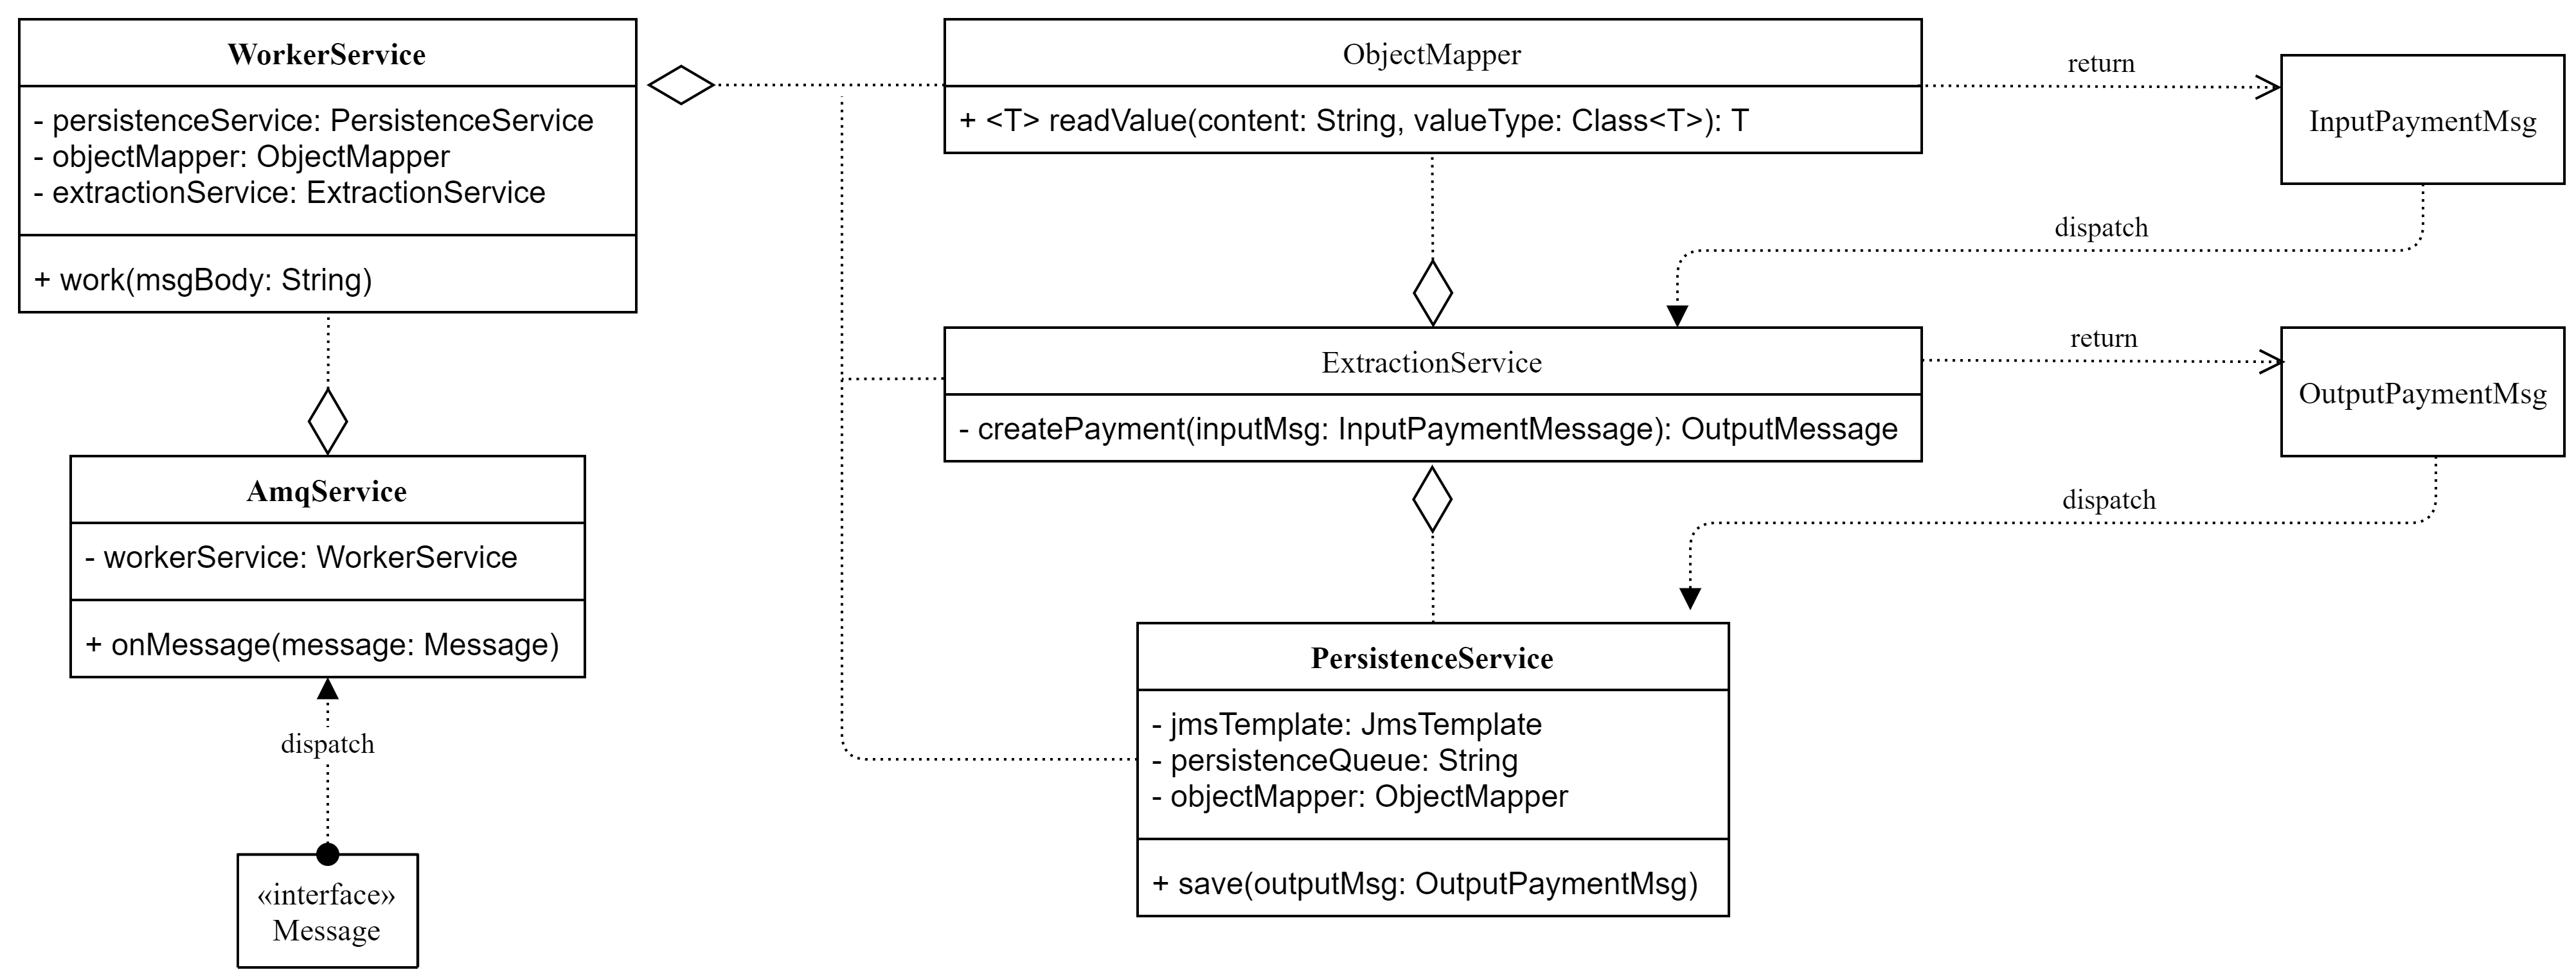
\includegraphics[width=\linewidth]{kapitel/problemloesung/implementierung/_img/consumer-uml}
	\caption[Consumer UML]{Consumer UML}
	\label{fig:consumerUml}
\end{figure}

Der Einstiegspunkt für den Spring-Konsumenten stellt der \emph{AmqService} dar. Nachrichten werden mithilfe dieser Komponente aus der Warteschlange des ActiveMq Brokers ausgelesen und an den \emph{WorkerService} delegiert. Über eine \emph{ObjectMapper} Instanz wird aus dem übergebenen String eine Objektinstanz eines Datenobjektes (\emph{InputPaymentMessage}) generiert (siehe Listing \ref{lst:consumerLogic}). Dieses Objekt wird an einen weiteren Service übergeben, der ein Element entsprechend der Vorgaben im Datenobjekt extrahiert. Wenn das zugrunde liegende XML nicht XSD-konform ist oder das Element zum spezifizierten Pfad nicht gefunden werden kann, wird eine Null-Referenz ausgegeben. Es folgt ein Nullcheck, bevor die Nachricht der Persistenzschicht übergeben wird.

\begin{lstlisting}[style=javaStyle,caption={WorkerService - Consumer Logik},label=lst:consumerLogic]

  ...

  @SneakyThrows
  public void work(String msgBody) {
    InputPaymentMsg inputMessage = objectMapper.readValue(msgBody, InputPaymentMsg.class);
    OutputPaymentMsg outputMessage = extractionService.createPayment(inputMessage);
    if (outputMessage != null) {
      persistenceService.save(outputMessage);
    }
    Thread.sleep(3000);
  }

  ...

\end{lstlisting}

\newpage

\subsection{Prometheus}

\paragraph{Regelsatz für Skalierung}
Prometheus ist eine Komponente, die zum Monitoring und zur Steuerung der Skalierung genutzt werden kann (siehe Abschnitt \ref{ss:prometheus} \nameref{ss:prometheus}). Für dieses Projekt musste diese lediglich derartig konfiguriert werden, dass entsprechende Alerts generiert werden und an die Alter-Manager-Komponente weitergeleitet werden können. Diese Komponente informiert erst anschließend die (Proxy-)Scaler-Komponente. Die auszuwertenden Regeln residieren jedoch bereits in der Prometheus Komponente. Das Regelwerk wurde nach folgendem Schema entworfen:

\bigskip

\begin{minipage}{\linewidth}
\begin{tabularx}
  {\textwidth}
  { X | X | X | X | X }
  \toprule
      \centering \hspace{4mm} \uline{QL3} \newline \footnotesize \textit{QB2 \textless{} MC} 
    & \centering \hspace{4mm} UP \newline \footnotesize \textit{abs(CB0 -- CB3)} 
    & \centering \hspace{4mm} UP \newline \footnotesize \textit{abs(CB1 -- CB3)} 
    & \centering \hspace{4mm} UP \newline \footnotesize \textit{abs(CB2 -- CB3)} 
    & \centering \hspace{4mm} OK \newline -- 
    \tabularnewline
  \hline
      \centering \hspace{4mm} \uline{QL2} \newline \footnotesize \textit{QB1 \textless{} MC $\leq$ QB2} 
    & \centering \hspace{4mm} UP \newline \footnotesize \textit{abs(CB0 -- CB2)} 
    & \centering \hspace{4mm} UP \newline \footnotesize \textit{abs(CB1 -- CB2)} 
    & \centering \hspace{4mm} OK \newline -- 
    & \centering \hspace{4mm} DOWN \newline \footnotesize \textit{abs(CB2 -- CB3)} 
    \tabularnewline
  \hline
      \centering \hspace{4mm} \uline{QL1} \newline \footnotesize \textit{QB0 \textless{} MC $\leq$ QB1} 
    & \centering \hspace{4mm} UP \newline \footnotesize \textit{abs(CB0 -- CB1)} 
    & \centering \hspace{4mm} OK \newline -- 
    & \centering \hspace{4mm} DOWN \newline \footnotesize \textit{abs(CB1 -- CB2)} 
    & \centering \hspace{4mm} DOWN \newline \footnotesize \textit{abs(CB1 -- CB3)} 
    \tabularnewline
  \hline
      \centering \hspace{4mm} \uline{QL0} \newline \footnotesize \textit{MC $\leq$ QB0} 
    & \centering \hspace{4mm} OK \newline -- 
    & \centering \hspace{4mm} DOWN \newline \footnotesize \textit{abs(CB0 -- CB1)} 
    & \centering \hspace{4mm} DOWN \newline \footnotesize \textit{abs(CB0 -- CB2)} 
    & \centering \hspace{4mm} DOWN \newline \footnotesize \textit{abs(CB0 -- CB3)} 
    \tabularnewline
  \hline
    & \centering \hspace{4mm} \uline{CL0} \newline \footnotesize \textit{CB0 == CC} 
    & \centering \hspace{4mm} \uline{CL1} \newline \footnotesize \textit{CB0 \textless{} CC $\leq$ CB1} 
    & \centering \hspace{4mm} \uline{CL2} \newline \footnotesize \textit{CB1 \textless{} CC $\leq$ CB2} 
    & \centering \hspace{4mm} \uline{CL3} \newline \footnotesize \textit{CB2 \textless{} CC $\leq$ CB3} \tabularnewline
  \bottomrule
\end{tabularx}
\end{minipage}

\bigskip

Diese Tabelle bestimmt das Skalierungsverhalten des Systems. Aus ihr werden die Regeln für die Prometheus-Konfiguration abgeleitet. Um diese Tabelle etwas anschaulicher erläutern zu können, werden die folgenden Werte für entsprechende Umgebungsvariablen angenommen. 


\begin{verbatim}
  CB0=1    CB2=10    QB0=15    QB2=100    CC: Container Count
  CB1=5    CB3=30    QB1=30               MC: Message Count
\end{verbatim}


Auf der horizontalen Achse wird die aktuelle Containeranzahl eines Systems in verschiedene Zustände eingeteilt. \emph{CL0} bis \emph{CL3} beschreibt hierbei das sogenannte \emph{Container Level}. Diese Level geben Abschnitte an, in denen sich die Containeranzahl zum aktuellen Zeitpunkt befinden kann. Diese Grenzen wurde, mithilfe von Variablen festgelegt und mit dem Kürzel \emph{CB0} bis \emph{CB2} versehen, dies steht für den Begriff "\emph{Container Bound}". Die aktuelle Containeranzahl (engl. \emph{Container Count}) selbst wurde in der Tabelle mit \emph{CC} abgekürzt. Wenn im System zu einem betrachteten Zeitraum beispielsweise fünf Containerinstanzen einer Konsumenten-Komponente laufen (im nachfolgenden stets als \emph{Consumer-Container} bezeichnet), dann befindet sich das System im Zustand \emph{Container Level 1}, da die untere Grenze des Intervalls mit \emph{CB0} auf 1 und die obere auf 5 gesetzt wurde. 

Eine ähnliche Eingrenzung gibt es ebenfalls bezüglich der vertikalen Achse, wobei die unbeantworteten Nachrichten einer Warteschlange in einem Message-Broker betrachtet werden. Hierbei steht das \emph{QL0} bis \emph{QL3} für das sogenannte "\emph{Queue Level}". Über die \emph{Queue Bound} (kurz \emph{QB0} bis \emph{QB3}) werden hierbei die Grenzen der Intervalle festgelegt. Wenn beispielsweise 101 unbeantwortete Nachrichten in der Warteschlange residieren, befindet sich das System im Zustand \emph{QL3}, da die \emph{Queue Count} (kurz \emph{QC}) größer ist als die Grenze \emph{QB2} (festgelegt auf 100).

Aus einer Überkreuzung dieser beiden Informationen lässt sich ableiten wie das System skaliert werden soll. Um beim beschriebenen Beispiel zu bleiben, würde sich das System im Feld \emph{CL1QL3} befinden. Hierbei gibt es zu wenig Container für die gegebene Nachrichtenanzahl. Die Containeranzahl muss demnach nach oben skaliert werden und zwar um die Differenz der beiden Container-Intervall-Grenzen \emph{CB1} und \emph{CB3}. Wenn diese Skalierung durchgeführt wurde, befindet sich das System anschließend im Zustand \emph{CL3QL3}. Die Hauptdiagonale der Tabelle beschreibt die Idealzustände; hierbei muss keine weitere Skalierung vorgenommen werden. 

\label{prometheus:skalierungsmechanismus}
Ein wesentlicher Nachteil dieser Herangehensweise ist, dass das System beim Skalieren über mehrere Intervallgrenzen hinweg mit mehreren Zellen in Berührung kommt. So befindet sich das System bei der beschriebenen Skalierung beispielsweise für einen Moment im Zustand \emph{CL2QL3}. Je nach Konfiguration des Systems schlägt diese Regel hierbei an, selbst wenn sich das System bereits in einem Skalierungsprozess befindet. Es gibt mehrere Möglichkeiten dieses Problem zu umgehen. Es ist zum Beispiel möglich das zeitliche Anfragenintervall durch Steuerungsinformationen vom Broker zu erhöhen, in der Hoffnung, dass das System bereits die gezielte Containeranzahl erreicht hat, sobald die nächste Anfrage erfolgt. Dies hat allerdings zur Folge, dass das System generell sehr lange braucht um zu erkennen, ob eine Skalierung bei der nächsten Aktion nötig ist oder nicht. Da dies einen unpraktikablen Ansatz darstellt, wurde diese Verantwortlichkeit an den Proxy-Scaler übergeben. Da diese Proxy-Komponente die tatsächlichen Skalierungsanfragen an die Docker-Scaler-API navigiert, ist sie ebenfalls in der Lage entsprechende Nachrichten zurückzuhalten, wenn klar ist, dass es sich hierbei um einen "\emph{Fehlalarm}" handelt, bei dem lediglich eine Skalierungsstufe während eines bereits laufenden Prozesses durchlaufen wird. 

Ein Satz Sonderregeln, die bisher nicht erwähnt wurden, betreffen den Initialisierungszustand. Hierbei wird geprüft, ob die Minimalanzahl von Containern läuft. Falls dies nicht der Fall sein sollte, wird eine Skalierungsanfrage für genau diese Anzahl generiert.


\paragraph{Konfiguration}

\begin{lstlisting}[style=bashStyle,caption={Umgebungsvariablen - Prometheus Regelsatz},label=lst:envMatrix]
  groups:
  - name: springScaleAlert
    rules:
      - alert: spring_baseline
        expr: >
          org_apache_activemq_Broker_ConsumerCount{
            brokerName="localhost",
            destinationName="${AMQ_SPRING_QUEUE_NAME}", 
            destinationType="Queue",
            instance="activemq:8080", 
            job="services"
          } < ${SCALING_CB0} 

  ...

\end{lstlisting}

Dieser Ausschnitt aus dem hinterlegten Regelwerk stellt die als letztes erwähnte Sonderregel für die minimale Containeranzahl dar. Hiermit wird beispielhaft beschrieben, wie die erläuterten Regeln aus der Tabelle codiert werden. Das Schlüsselwort \emph{groups} dient allein dazu verwandte Regeln zusammenzufassen. Der Rest ist selbsterklärend. Erwähnenswert ist, dass der Wert des Schlüssels \emph{alert} in dieser Form ohne Modifikationen an den Alert-Manager weitergeleitet und dort entsprechend verarbeitet wird.

Im folgenden Listing ist die Dateistruktur der Konfigurationsdateien von Prometheus dargestellt.

\begin{lstlisting}[style=bashStyle,caption={Prometheus -- Konfigurationsstruktur},label=lst:envMatrix]
  $ tree stack/data/prometheus/ --charset=ascii
  stack/data/prometheus/
  |-- alert-unparsed.yml
  |-- alert.yml
  |-- prometheus.yml
  `-- targets
      `-- alertmanager.json
\end{lstlisting}

In der Datei "\emph{alert-unparsed.yml}" werden die Regeln nach der bisher beschriebenen Struktur abgelegt. Hierbei wurden keinerlei feste Werte für die Intervallgrenzen eingesetzt. Zur Laufzeit der Komponente ist dies allerdings nicht zulässig. Um dennoch die Flexibilität des Formats mit Umgebungsvariablen nutzen zu können wurde ein Skript verfasst, das vor dem Starten der Komponente ausgeführt wird und die Datei "\emph{alert.yml}" generiert. Bei Ausführung des Skripts werden die hinterlegten Werte der Umgebungsvariablen in das gegebene Skript eingesetzt\footnote{Datei:\\\url{https://github.com/derMacon/serverless-bsc-thesis/blob/main/anhang/refs/alert-unparsed.yml}}. 

In der "\emph{prometheus.yml}" Datei befindet sich ein Eintrag, der dem System mitteilt, dass diese generierte Datei für die Regelauswertung verwendet werden soll. In der \emph{prometheus.yml} Datei werden ansonsten weitere Einstellungen bezüglich des Scraping-Intervalls, der Adressierung der zu überwachenden Komponenten sowie die Angabe des Namens des Alert-Managers konfiguriert\footnote{Datei: \url{https://github.com/derMacon/serverless-bsc-thesis/blob/main/anhang/refs/prometheus.yml}}.

Der Ordner \emph{target} enthält die Routing-Konfiguration für die Anbindung der generierten Alerts zur Alert-Manager-Komponente.
\subsection{Alter-Manager}
Diese Komponente ist in diesem Projekt sehr unkompliziert gehalten. Es wird lediglich ein Webhook erstellt, an den erhaltene Alerts ohne jegliche Modifikation weitergeleitet werden. Die komplette Konfiguration der Komponente ist unter folgender Url einsehbar: \url{https://github.com/derMacon/serverless-bsc-thesis/blob/main/anhang/refs/alertmanager.yml}


\subsection{Scaler Proxy}

Im folgenden UML-Diagramm (siehe Abbildung \ref{fig:proxyScalerUml} \nameref{fig:proxyScalerUml}) wird die grundlegende Klassenstruktur der Scaler-Proxy-Komponente zusammengefasst. 

\begin{figure}[ht!]
	\centering
	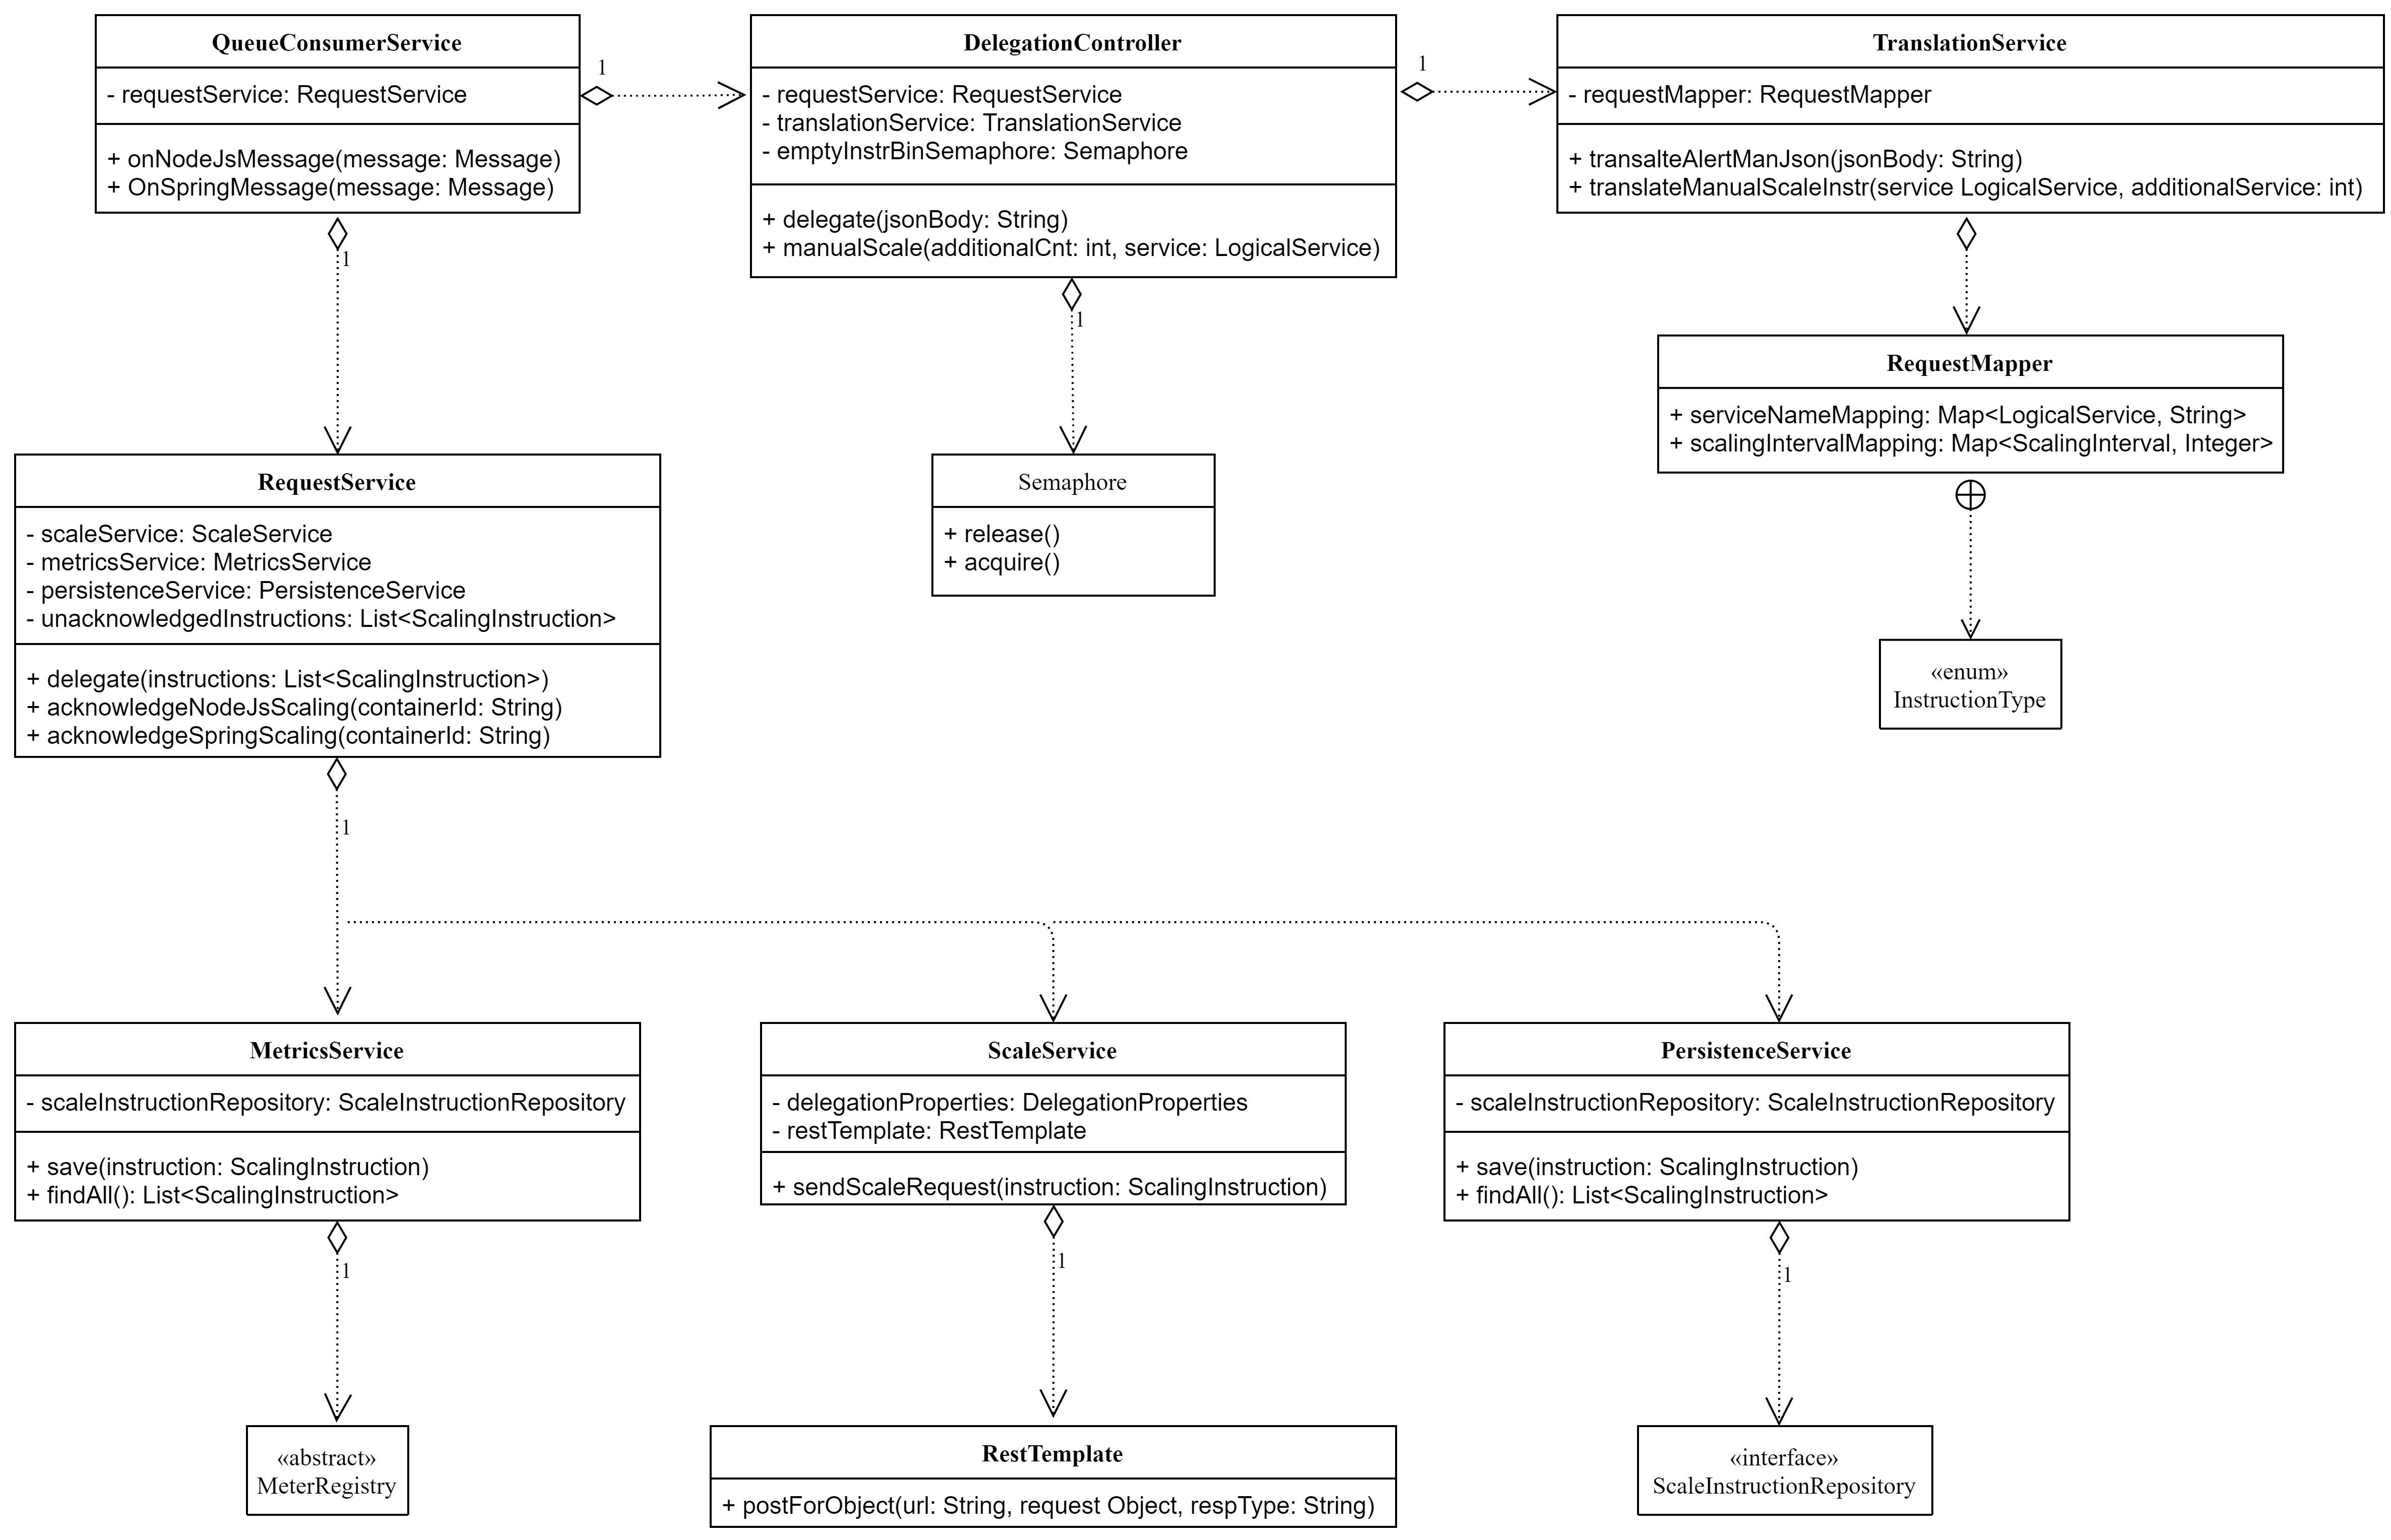
\includegraphics[width=\linewidth]{kapitel/problemloesung/implementierung/_img/scaler-proxy-uml}
	\caption[Scaler-Proxy UML]{Scaler-Proxy UML}
	\label{fig:proxyScalerUml}
\end{figure}

Diese Komponente stellt sowohl die Funktionalität bereit, Alerts vom Alert-Manager, als auch direkte Skalierungsanfragen vom Benutzer selbst anzunehmen. Für beide Szenarien gibt es einen entsprechenden Endpunkt. Beide Typen von Anfragen werden intern allerdings erst in ein Zwischenformat überführt, das wiederum vom \emph{RequestService} interpretiert werden kann. Die wesentliche Kernfunktionalität dieses Services wurde in Listing \ref{lst:proxyDelegate} \nameref{lst:proxyDelegate} dargestellt. Bei der Implementierung des Regelwerks in der Prometheus-Komponente wurde erwähnt, dass es einen Mechanismus zum Skalieren über mehrere Stufen des Models von der Proxy-Komponente geben muss (siehe Abschnitt \ref{prometheus:skalierungsmechanismus} \nameref{prometheus:skalierungsmechanismus}). Dies wurde in der Proxy-Komponente über ein Acknowledgement der einzelnen hochgefahrenen Container ermöglicht. Es wird intern eine Liste von Skalierungsinstruktionen verwaltet. Jeder Container, der im Zuge einer der Instruktionen gestartet wird, generiert eine ID, die diesen Container identifiziert und gibt diese dem Proxy-Service über eine REST-Schnittstelle bekannt. Dadurch kann die Proxy-Komponente festzustellen, ob sich das System aktuell in einem Skalierungsprozess befindet oder nicht. Wenn nun neue Skalierungsinstruktionen eingespeist werden (zum Beispiel in einer der beschriebenen Übergangsphasen in der Tabelle), dann ist es der Komponente möglich, mithilfe einer einfachen Überprüfung der Liste diese zu verwerfen (Zeile 2). Im Anschluss wird über sämtliche generierten Skalierungsinstruktionen iteriert. Die verwaltete Liste wird mit neuen Einträgen gefüllt und die Anfragen werden an die Skalierungs-API geschickt, die als letztes Abstraktionslevel ohne weitere Funktionalität die Skalierung für den Benutzer übernimmt. 

\begin{minipage}{\linewidth}
\begin{lstlisting}[style=javaStyle,caption={Proxy Scaler -- RequestService},label=lst:proxyDelegate]
  public boolean delegate(List<ScalingInstruction> instructions) {
    if (!unacknowledgedInstructions.isEmpty()) {
        return false;
    }
    boolean scaledToMinRepl = false;
    for (ScalingInstruction instruction : instructions) {
        instruction.setReceivedRequestTimestamp(now());
        if (instruction.getScalingDirection() == UP) {
            unacknowledgedInstructions.add(instruction);
        }
        scaledToMinRepl = scaledToMinRepl || scaleService.sendScaleRequest(instruction);
    }
    return scaledToMinRepl;
  }
\end{lstlisting}
\end{minipage}

\subsection{Docker-Scaler}
Dieses Open-Source-Projekt\footnote{\url{https://thomasjpfan.github.io/docker-scaler}} bietet eine REST-Schnittstelle, über die es möglich ist, einen zugrunde liegenden Docker-Swarm zu skalieren. Die komplette Anfrage kann innerhalb einer einzigen POST-Anfrage abgeschickt werden. In diesem Projekt wurde hierfür der folgende Endpunkt verwendet:

\begin{itemize}
  \item URL: /v1/scale-service
  \item Methode: POST
  \item Parameter:
  \begin{itemize}
    \item service: Name des zu skalierenden Services
    \item scale: Richtung in die skaliert werden soll 
    \item by: Anzahl zusätzlicher / überflüssiger Replicas
  \end{itemize}
\end{itemize}

\subsection{Grafana}

Dieses Werkzeug wird zur Erstellung von Graphen hinsichtlich erhaltener Metriken verwendet. Diese Daten werden von allen relevanten Stack-Komponenten über eine einheitliche Schnittstelle bereitgestellt und im Prometheus Client gebündelt. In der Grafana-Komponente wird hierbei lediglich die Prometheus-Komponente als \emph{Datasource} deklariert, um Zugriff auf diese Metriken zu erhalten \cite[Seite~99 ff.]{oreillyPrometheus}. In Abbildung \ref{fig:prometheusDatasource} \nameref{fig:prometheusDatasource} ist diese Konfiguration in Auszügen zu erkennen. Hierbei wird im Wesentlichen die Netzwerk-Adresse sowie der Port spezifiziert. 

\begin{figure}[ht!]
	\centering
	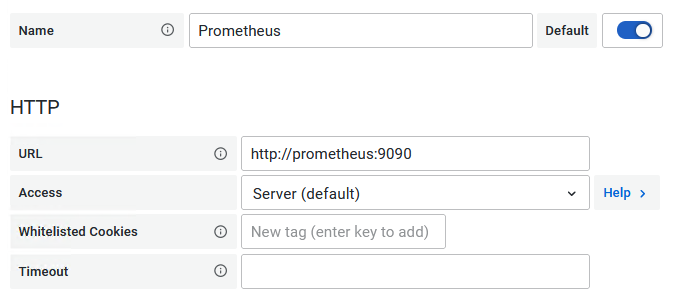
\includegraphics[width=.9\linewidth]{kapitel/problemloesung/implementierung/_img/prometheus-datasource}
	\caption[Prometheus - Datasource]{Prometheus - Datasource}
	\label{fig:prometheusDatasource}
\end{figure}

Über die in Prometheus deklarierten \emph{Targets} (überwachten Komponenten) können die wichtigsten Informationen ausgelesen werden. Die Abbildung \ref{fig:grafanaOverview} \nameref{fig:grafanaOverview} zeigt hierbei auf, wie das fertige Dashboard aussieht. Die Aufnahme wurde zum Zeitpunkt der Benchmarks-Tests, die als Grundlage für diese Analyse verwendet wurden, getätigt. Es lassen sich alle Metriken der Ergebnisanalyse (siehe Abschnitt \ref{ch:ergebnisanalyse} \nameref{ch:ergebnisanalyse}) in diesem Dashboard wiederfinden. 

\begin{figure}
	\centering
	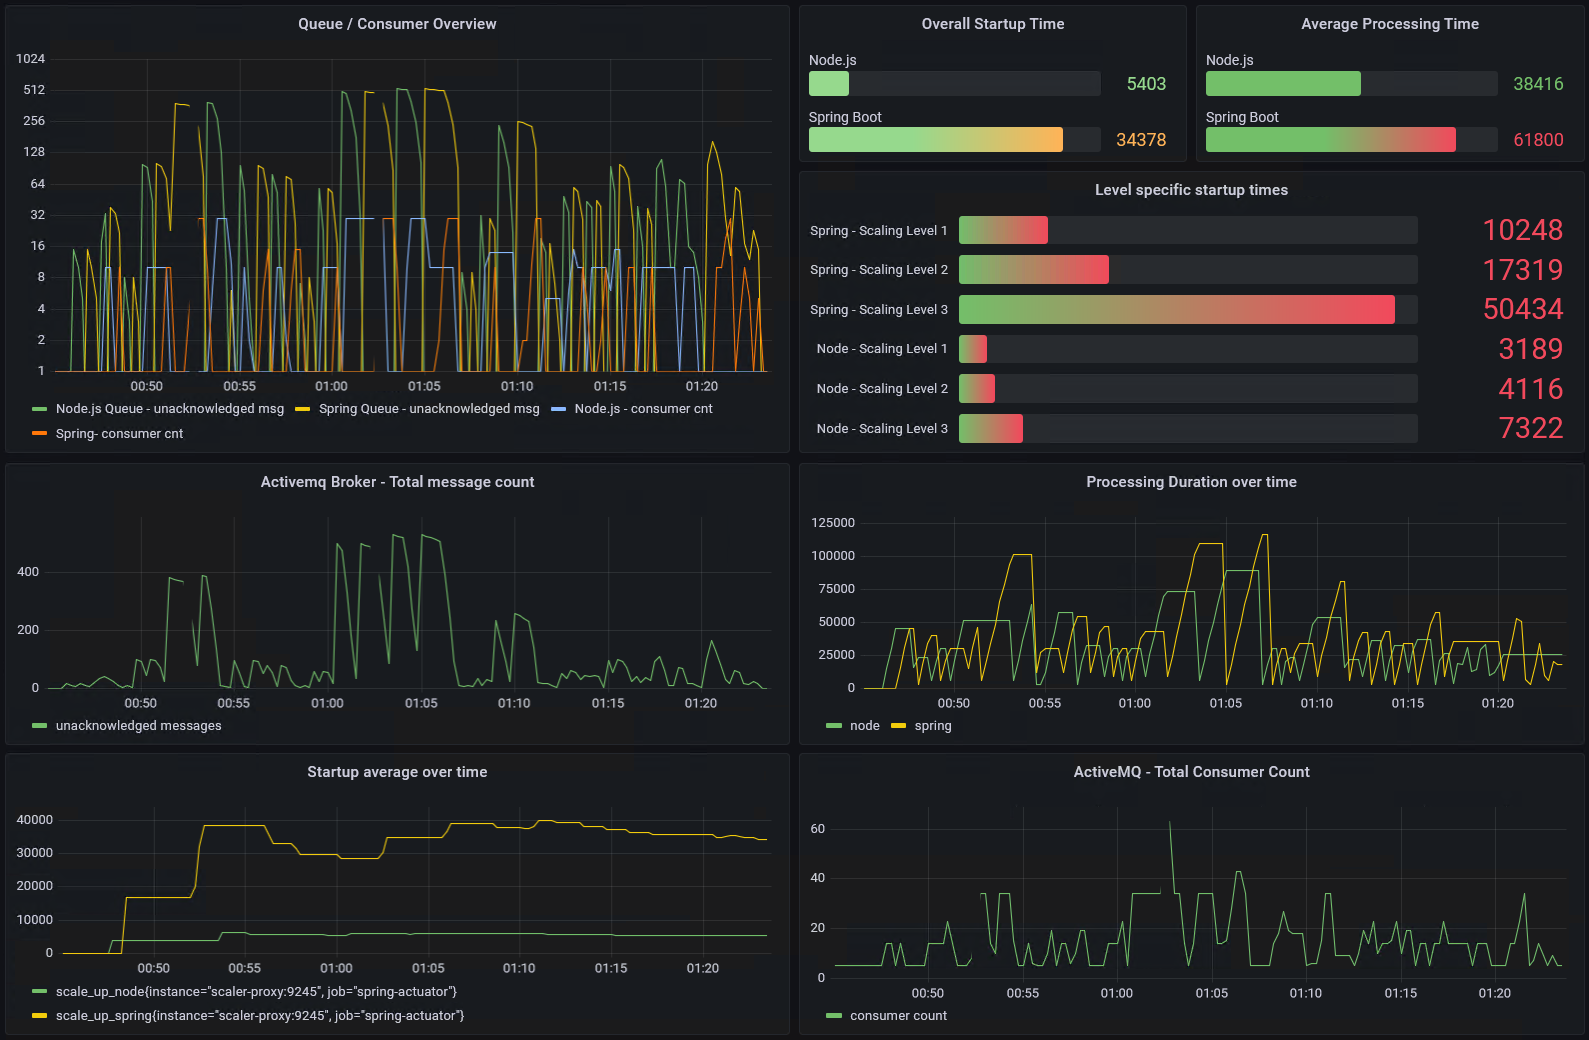
\includegraphics[width=\linewidth]{kapitel/problemloesung/implementierung/_img/grafana-dashboard-01}
	\caption[]{Grafana Dashboard}
	\label{fig:grafanaOverview}
\end{figure}

Um ein Dashboard zu erstellen, wird auf das Webinterface der Komponente selbst zugegriffen. Es gibt hierbei zwar auch die Möglichkeit Dashboards im JSON-Format einzulesen sowie zu exportieren, der Einfachheit halber wurde in diesem Projekt allerdings hierauf verzichtet. In der folgenden Abbildung ist zu erkennen, wie die Konfiguration einer Dashboard-Komponente über das Webinterface funktioniert (siehe Abbildung \ref{fig:grafanaPromQl} \nameref{fig:grafanaPromQl}). 

\begin{figure}
	\centering
	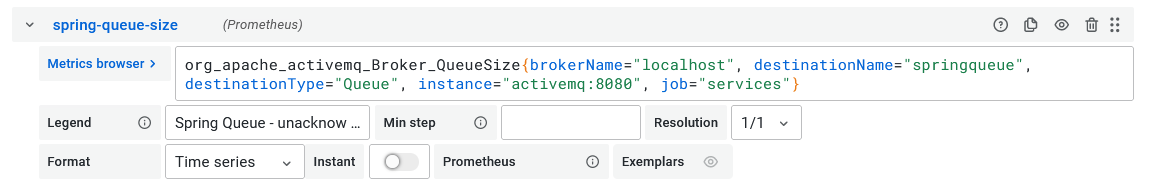
\includegraphics[width=\linewidth]{kapitel/problemloesung/implementierung/_img/grafana-promql}
	\caption[]{Grafana - Graphenkonfiguration}
	\label{fig:grafanaPromQl}
\end{figure}

Das wesentliche Formularelement, das während der Konfiguration verwendet wird, stellt die Anfrage an die definierte Datasource dar (engl. \emph{query}). Hierbei wird auf eine Anfragesprache namens \emph{PromQL} zurückgegriffen um verschiedene Metriken auslesen zu können. In der Abbildung ist beispielsweise zu erkennen, dass bei einem Messagebroker mit dem Namen "\emph{localhost}" eine Warteschlange (engl. \emph{queue}) mit dem Namen "\emph{springqueue}" mit der Adresse "\emph{activemq:8080}" die aktuelle Größe der Warteschlange ausgeben soll\footnote{Die hier genutzte Anfrage lässt sich zum Beispiel bei der ActiveMq-Dokumentation nachlesen: \url{https://docs.splunk.com/Observability/gdi/activemq/activemq.html}}. Diese Anfrage wird in einem konfigurierbaren Intervall wiederholt (hier alle 15 Sekunden). Es ist auch möglich mehrere Anfragen pro Graph zu definieren um mehrere Werte gegenüberzustellen sowie mehrere Anfrageergebnisse zu verknüpfen. Die erhaltenen Daten werden anschließend automatisch in einem Graphen dargestellt (siehe Abbildung \ref{fig:graphEx} \nameref{fig:graphEx}). 

\begin{figure}
	\centering
	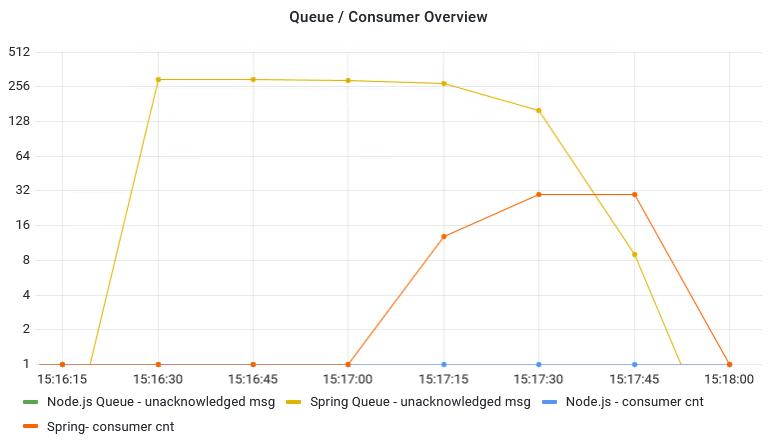
\includegraphics[width=.8\linewidth]{kapitel/problemloesung/implementierung/_img/grafana-graphExample}
	\caption[]{Grafana - Beispielhafter Graph}
	\label{fig:graphEx}
\end{figure}

In diesem Beispiel wurde eine größere Menge von Nachrichten für den Spring-Konsumenten in die Warteschlange geladen. Die unbeantworteten Nachrichten wurden hierbei in Gelb dargestellt. Da zum Start der Anwendung nur ein einziger Container des Services aktiv läuft, werden im Nachhinein weitere Container hochgefahren (siehe orange Kurve). Es ist zu erkennen, dass die Nachrichtenanzahl zu Anfang sehr langsam abnimmt, mit ansteigender Containeranzahl jedoch immer schneller sinkt.

Die Daten hinsichtlich der Node.js Komponenten sowie die Zahlenwerte für die gemessenen Start-up-Zeiten werden gleichermaßen in eigenen Dashboard-Komponenten dargestellt. Da die Konfiguration der bereits Vorgestellten allerdings deutlich ähnelt, wurde hierbei darauf verzichtet diese ebenfalls zu erläutern. Da das Dashboard im Allgemeinen einen eher überprüfenden Charakter einnimmt um nachvollziehen zu können wie die letztendlichen Messwerte berechnet wurden, ist diese gesamte Komponente auch von untergeordneter Bedeutung.

\section{Deployment auf der Containerplattform}
Nachdem im letzten Abschnitt beschrieben wurde, wie die einzelnen Stack-Komponenten implementiert wurden, wird im Folgenden auf das Deployment mithilfe von Containern im Docker-Swarm-Stack eingegangen. 

\subsection{Build}
Hierbei werden zuerst die Buildvorgänge der einzelnen Komponenten beschrieben, im Anschluss daran wird ein Überblick über die Orchestrierung des Stacks gegeben.

\subsubsection{Spring Komponenten}

Um das Projekt im Komponenten-Stack als Dockercontainer zu deployen, muss in einem ersten Schritt ein Docker-Image erstellt werden. Dieses kann im Anschluss als Container instanziiert werden. Zum Erstellen eines Docker-Images wird auf ein sogenanntes "\emph{Dockerfile}" zurückgegriffen, das die Beschreibung des Build-Prozesses für dieses Image enthält. Da alle Spring-Projekte im Komponenten-Stack mit einem fast identischen Dockerfile versehen wurden, gilt die anschließende Erläuterung in gleichem Maß für alle Spring-Projekte dieses Stacks.

Damit die folgende Erklärung der genutzten Dockerfiles verständlich dargestellt werden kann, folgt eine kurze Zusammenfassung der Struktur eines Docker-Images. "\emph{A Docker image is made up of filesystems layered over each other}" \cite[Seite~71]{turnbulldocker}. Als erste Schicht wird hierbei ein bootbares Filesystem eingeführt, das einem typischen Linux-Bootsystem ähnelt. Anschließend kann dieses Modell mit weiteren Schichten erweitert werden. Hierfür wird der sogenannte "\emph{union mount}" Mechanismus verwendet, der es ermöglicht mehrere read-only Dateisysteme in das Root-Dateisystem zu integrieren. Bei einem neu hinzugefügten Dateisystem ist es möglich auf die Unterordner der vorher hinzugefügten Systeme zuzugreifen. In einer Docker-Umgebung spricht man bei diesen aufgeschichteten Dateisystemen von Docker-Images. "\emph{Images can be layered on top of one another.  The image below is called the parent image and you can traverse each layer until you reach the bottom of the image stack where the final image is called the base image.  Finally, when a container is launched from an image, Docker mounts a read-write filesystem on top of any layers below. This is where whatever processes we want our Docker container to run will execute}" \cite[Seite~71]{turnbulldocker}. In Abbildung \ref{fig:dockerImage} wurde dies auch noch einmal grafisch aufgearbeitet.

\begin{figure}[ht!]
	\centering
	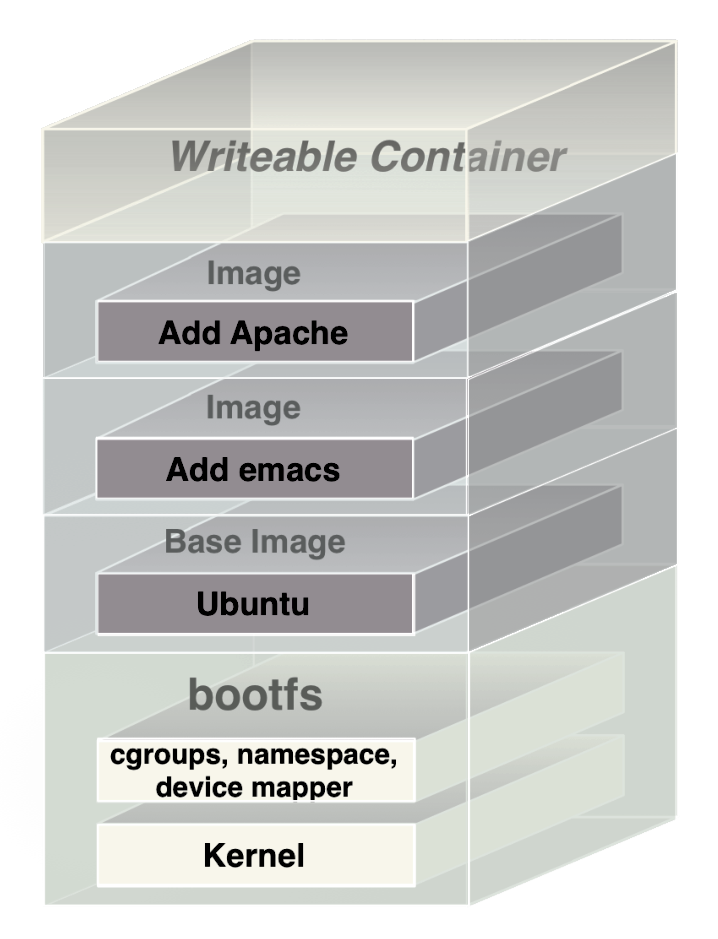
\includegraphics[width=.6\linewidth]{kapitel/problemloesung/implementierung/_img/docker-image-fig}
	\caption[Docker Image -- Schaubild]{Docker Image -- Schaubild \cite[Seite~72]{turnbulldocker}}
	\label{fig:dockerImage}
\end{figure}

Um ein Docker-Image zu erstellen, wurde bei diesem Projekt auf eine Beschreibungsdatei namens "\emph{Dockerfile}" zurückgegriffen.

\begin{minipage}{\linewidth}
\begin{lstlisting}[style=javaStyle,caption={Dockerfile - Supplier},label=lst:supplierDockerfile]
  FROM maven:3.8.1-openjdk-11 AS build
  COPY src /usr/src/app/src
  COPY pom.xml /usr/src/app
  RUN mvn -f /usr/src/app/pom.xml clean package -DskipTests

  FROM gcr.io/distroless/java
  COPY --from=build /usr/src/app/target/supplier-backend.jar /usr/app/supplier-backend.jar
  EXPOSE 9245
  ENTRYPOINT ["java","-jar","/usr/app/supplier-backend.jar"]
\end{lstlisting}
\end{minipage}

\begin{itemize}

  \item Zeile 1: Ein Dockerfile beginnt mit der Angabe eines sogenannten "\emph{Baseimages}". Dies kann eine minimale Linux Distribution sein oder wie in diesem Fall ein System, auf dem bereits diverse Konfigurationen definiert wurden. Bei dem verwendeten Image wurde eine Java Runtime sowie das Buildprogramm \emph{Maven} bereits vorinstalliert. Beides wird für die Ausführung des Spring-Projekts gebraucht. 

  \item Zeile 2: Der Buildprozess wird in dem Root-Verzeichnis des Spring-Projekts ausgeführt. Hier befinden sich in einem Unterordner alle Quellcodedateien, die mit diesem Befehl in das \emph{usr} Verzeichnis des zu erstellenden Images kopiert werden. 
  
  \item Zeile 3: Da alle Spring-Projekte dieses Stacks mithilfe des Build-Tools \emph{Maven} gebaut werden, wird die \emph{pom.xml} Beschreibungsdatei aus dem Root-Verzeichnis ebenfalls in den Container kopiert. Diese Datei enthält alle wesentlichen Metainformationen des Projekts. Dazu gehören beispielsweise sämtliche Abhängigkeiten, verwendete Build-Plugins und Projektinformationen. 

  \item Zeile 4: Der Run-Befehl ermöglicht es, den nachfolgenden Shell-Befehl in einer Linux-Shell innerhalb des Containers selbst auszuführen. Hierbei wird die ausführbare .jar Datei gebaut, die im späteren Verlauf im Dateisystem deployed wird.

  \item Zeile 6: Es folgt eine erneute Anweisung zum Laden eines Base-Images, dies ist Teil eines sogenannten \emph{multi-stage} Builds. Wie im letzten Abschnitt erwähnt, werden beim Bauen von Docker-Images verschiedene Dateisysteme ineinander gemounted, hierbei entsteht eine Art Schichtenmodell. Bezogen auf ein Dockerfile wird mit jeder einzelnen Befehlszeile der Datei ein neues Image erstellt. Um  am Ende ein möglichst kleines Docker-Image zu erhalten, wird versucht diese Schichtanzahl so minimal wie möglich zu halten. Hierbei gibt es die Möglichkeit, das Bauen der ausführbaren Datei auszulagern und lediglich die fertige ausführbare Datei in den Container zu laden. Mit diesem Ansatz ist es allerdings nicht möglich, das Image direkt auf dem Server zu bauen, es sei denn die Datei liegt vor oder das System stellt alle notwendigen Buildwerkzeuge bereit. Dies ist sehr unpraktisch, weswegen in der Praxis hierbei ein sogenannter "\emph{multistage build}" verwendet wird \label{it:multiBuild} \cite[Kapitel~multi stage build]{docker-doc}. Hierbei kann auf einzelne Stufen Bezug genommen und spezifizierte Dateien von einem Image direkt in ein anderes kopiert werden. Bezogen auf das dargestellte Dockerfile, ist es möglich die ausführbare Datei des vorherigen Buildprozesses zu kopieren ohne sämtliche Metadaten, die bei dem Buildprozess anfallen, ebenfalls kopieren zu müssen.

  \item Zeile 7: Wie im letzten Schritt erwähnt, wird hierbei die ausführbare Datei vom Buildprozess in das aktuelle Image herüberkopiert. Hierfür wird sich des Schlüsselworts \emph{--from} bedient. Die vorher generierten Schichten, die im Buildprozess verwendet wurden, werden bei der Erstellung des letztendlichen Images wieder verworfen, da sie mit einem neuen Baseimage überschrieben wurden.

  \item Zeile 8: Der Port, über den sämtliche Kommunikation mit der Außenwelt stattfindet, wird freigegeben. 

  \item Zeile 9: Der Entrypoint ähnelt dem \emph{CMD}-Befehl stark, es ist zum Ausführungszeitpunkt des Containers allerdings schwieriger diesen zu überschreiben.

\end{itemize}


\paragraph{Anmerkung: Vorteile der Imageschichtung} Diese Schichtung der Images ermöglicht einen einfachen Caching-Mechanismus. Es müssen schließlich nur die Teile des Images neu gebaut werden, die sich tatsächlich geändert haben. Dazu wird die Schicht ermittelt, ab der eine erste Abweichung zum vorherigen Build festgestellt werden kann. Anschließend wird lediglich diese Schicht sowie alle Schichten darüber, neu gebaut. Die \emph{parent layer} werden allerdings wiederverwendet. Beim Erstellen von Images sollte daher Wert darauf gelegt werden, den dynamischen Teil des Buildvorgangs möglichst weit an das Ende eines Dockerfiles zu legen, um den Caching-Mechanismus der Docker-Engine bestmöglich auszunutzen.

\subsubsection{Node.js}

\paragraph{Überblick}
Das Node.js-Projekt wurde mithilfe des npx "\emph{create-react-app}"-Starters initialisiert. npx ist ein package runner für den node package manager (kurz npm). npx stellt dabei ein CLI-Werkzeug bereit, welches bei der Installation von npm direkt mit ausgeliefert wird und dient zur Unterstützung der Verwaltung von Abhängigkeiten. Im Bezug auf das Node.js-Projekt ist es beispielsweise möglich hiermit ein Projekt zu initialisieren, das auf der Programmiersprache \emph{Typescript} basiert und nicht wie herkömmlich, auf Javascript. Typescript stellt eine Erweiterung von Javascript dar, es ist demnach möglich Javascript-Code in einem Typescript-Projekt auszuführen. Es wurde sich in diesem Projekt für Typescript entschieden, da diese Sprache die vier wesentlichen Prinzipien objektorientierter Sprachen bereitstellt. Diese setzten sich aus der \emph{Kapselung von Code}, der \emph{Vererbung}, \emph{Abstraktion} und \emph{Polymorphie} zusammen \cite{typescript-oop}. Dies ermöglicht eine klarer strukturierte Codebasis und ist über ein objektorientiertes Modell ebenfalls einfacher mit dem Spring Boot Pendant zu vergleichen.

\paragraph{Kompilieren der Sourcen}
Ähnlich wie Java wird auch ein Typescript-Projekt kompiliert, hierbei wird jedoch Javascript-Code erzeugt. Die Konfiguration des Typescript-Compiler \emph{tsc} befindet sich in einer Datei namens \emph{tsconfig.json} (siehe Listing \ref{lst:tsconfig} \nameref{lst:tsconfig}).

\newpage

\begin{lstlisting}[style=javaStyle,caption={tsconfig.json},label=lst:tsconfig]
  {
  "compilerOptions": {

    /* Basic Options */
    "target": "es5",

    /* Specify ECMAScript target version: 'ES3' (default), 'ES5', 'ES2015', 'ES2016', 'ES2017', 'ES2018', 'ES2019', 'ES2020', or 'ESNEXT'. */
    "module": "commonjs",
    "outDir": "./dist",
    "rootDir": ".",

    /* Strict Type-Checking Options */
    "strict": true,
    "esModuleInterop": true,

    /* Advanced Options */
    "skipLibCheck": true,
    "forceConsistentCasingInFileNames": true
  }
}

\end{lstlisting}

Die wichtigsten Konfigurationsparameter im Überblick:

\begin{itemize}
  \item \emph{target}: Hierbei wird der Javascript-Standard angegeben, in den die Typescript-Quellen übersetzt werden sollen.
  \item \emph{outdir}: Das Ausgabeverzeichnis, in dem die übersetzten Javascript-Dateien abgelegt werden sollen.
  \item \emph{rootdir}: Das Root-Verzeichnis des Typescript-Projekts.
  \item \emph{strict}: Das Compilerflag hinsichtlich der Typisierung und sonstiger Javascript-Eigenheiten. Ersetzt die Notwendigkeit, in jeder einzelnen Quellcodedatei einen "\emph{use strict}" Befehl angeben zu müssen, um die Datei im ECMAScript \emph{strict mode} zu parsen\footnote{Für weitere Informationen siehe Typescript-Dokumentation \cite[Kapitel~tsconfig]{typescript-doc}.}.
\end{itemize}

Ähnlich wie bei einem Maven-Projekt eine \emph{pom.xml} Datei verwendet wird, um die Projekt-Konfigurationseinstellungen festzuhalten, wird bei einem Typescript-Projekt eine sogenannte \emph{package.json} erstellt (siehe Listing \ref{lst:package} \nameref{lst:package}). Die komplette Datei ist unter folgender URL einsehbar: \url{https://github.com/derMacon/serverless-bsc-thesis/blob/main/anhang/refs/package.json}

\newpage

\begin{lstlisting}[style=javaStyle,caption={Typescript -- package.json},label=lst:package]
  {
  "name": "node-consumer",
  "main": "index.js",
  "scripts": {
    "test": "echo \"Error: no test specified\" && exit 1",
    "build": "tsc"
  },
  "author": "hoffmann",

  ...

  "dependencies": {
    "@types/node": "^15.6.1",
    "@types/pg": "^8.6.0",
    "dotenv": "^10.0.0",
    "fs": "^0.0.1-security",
    "ini": "^2.0.0",
    "libxmljs2": "^0.27.0",
    "pg": "^8.6.0",
    "stompit": "^1.0.0",
    "typescript": "^4.3.2",
    "xmldom": "^0.6.0",
    "xpath": "^0.0.32"
  },
  "devDependencies": {
    "@types/ini": "^1.3.30"
  }
}
\end{lstlisting}

In dem angegebenen Dateiinhalt lassen sich vor allem Metainformationen des Projekts identifizieren (Projektname, Autor). Außerdem werden Projekt-Abhängigkeiten definiert, wobei die letztendlich genutzten Packages mit den entsprechenden Versionsnummern in einem dedizierten Format aufgezählt werden. Diese sind standardmäßig Javascript Projekte. Da Typescript dennoch die Möglichkeit bietet, über einen definierten \emph{any type} eine untypisierte Variante von Variablen etc. zu erstellen, können diese Bibliotheken ohne weitere Konfiguration genutzt werden. Um allerdings die Typisierungsfunktionen von Typescript sinnvoll nutzen zu können, müssen diese Informationen entweder als getrennte Abhängigkeit importiert werden (siehe Zeile 13 / 14) oder sie sind bereits in der importierten Bibliothek enthalten und können nativ genutzt werden. Zur Überprüfung kann die Ausgabe des tsc-Compilers hinzugezogen werden.

\paragraph{Dockerbuild}
Um ein Dockerimage für das Typescript-Projekt zu erstellen, wird auf folgendes Dockerfile zurückgegriffen (siehe Listing \ref{lst:ts-dockerfile} \nameref{lst:ts-dockerfile}).

\newpage

\begin{lstlisting}[style=bashStyle,caption={Dockerfile - Typescript Projekt},label=lst:ts-dockerfile]
  # stage 1 building the code
  FROM node:10.15.3 AS builder
  WORKDIR /usr/app
  COPY package*.json ./
  RUN npm install
  COPY . .
  RUN npm run build 

  # stage 2
  FROM node:10.15.3-alpine
  WORKDIR /usr/app
  COPY package*.json ./
  RUN npm install --production
  COPY --from=builder /usr/app/dist ./dist
  COPY --from=builder /usr/app/schema.sql .
  COPY --from=builder /usr/app/specification.xsd .
  CMD node dist/src/index.js
\end{lstlisting}

Dieses ähnelt dem der Spring-Boot-Projekte (siehe Abschnitt \ref{ss:springProj} \nameref{ss:springProj}). Es werden ausführbare Quellen erstellt, die wiederum in einem zweiten Build-Schritt des \emph{multistage}-Buildverfahrens (siehe Abschnitt \ref{it:multiBuild} \nameref{it:multiBuild}) verwendet werden. Der wesentliche Unterschied beim ersten Schritt besteht darin, dass nicht eine einzelne ausführbare Datei erstellt wird, sondern die entsprechenden Javascript-Verzeichnisse generiert werden. Hierzu werden alle für den Build relevanten Typescript- und sonstigen Quellen in einem Zwischenschritt in einem Containerimage abgelegt. Anschließend erfolgt der Compileraufruf. Im zweiten Schritt werden lediglich die relevanten Quellen herüberkopiert und der Rest verworfen. 


\subsection{Komponentenstack}
Um den Stack zu starten wird auf verschiedene Skripte sowie Beschreibungsdateien zugegriffen. Im Folgenden wird erst die Beschreibung des Container-Netzwerks und anschließend der Build- sowie Start-Vorgang des Projekts beschrieben.

\subsubsection{Docker-Compose}
\paragraph{Einleitung}
Es ist möglich, ein Netzwerk von Containern manuell über das CLI der Docker-Engine zu starten, hierbei können Mounts bestimmter Verzeichnisse angelegt, Kommunikations-Netzwerke definiert und Ports freigegeben werden. Mithilfe von Shell-Skripten wäre es möglich, diese Schritte zu automatisieren. Dieses Vorgehen erscheint aber schon bei kleineren Projekten sehr unpraktisch und unübersichtlich, hierbei wird daher auf Werkzeuge wie zum Beispiel \emph{Docker-Compose}\footnote{\url{https://github.com/docker/compose}} zurückgegriffen. Dieses Tool bietet die Möglichkeit, über eine Beschreibungssprache einen Stack zu definieren, in dem sämtliche Abhängigkeiten bereits aufgelöst werden können. 

\paragraph{Container Networking}
Container werden hierbei in Clustern organisiert, die es ermöglichen, mithilfe des \emph{Docker-Link}-Mechanismus die Container über ein definiertes Netzwerk miteinander in Verbindung treten zu lassen. "\emph{The Docker server acts as a virtual bridge and the containers are clients behind it}" \cite[Seite~13]{oreilly-docker}. Jeder Container besitzt ein eigenes virtuelles Ethernet Interface, das eine eigene IP-Adresse allokiert und mit der beschriebenen Docker-Bridge verbunden ist. "\emph{Docker lets you bind ports on the host to the container so that the outside world can reach your container}" \cite{oreilly-docker}. Hierbei wird ein lokales Netzwerk allokiert, über das alle Container direkt miteinander kommunizieren können.

\paragraph{Stack-Konfiguration}
Um beim Beispiel des \emph{Suppliers} zu bleiben, folgt eine kurze Zusammenfassung der Stack-Konfiguration für den Spring-Supplier-Container (siehe Listing \ref{lst:dockerCompose} \nameref{lst:dockerCompose}). Die gesamte Docker-Compose Konfigurationsdatei befindet sich ebenfalls im Anhang\footnote{siehe \\ \url{https://github.com/derMacon/serverless-bsc-thesis/blob/main/anhang/refs/docker-compose.yml}}.

\begin{lstlisting}[style=bashStyle,caption={Docker Compose - Ausschnitt Supplier Definition},label=lst:dockerCompose]
  ...

  supplier-backend:
    image: supplier-backend
    build: supplier-backend/
    ports:
      - "${SUPPLIER_BACKEND_PORT}:${SUPPLIER_BACKEND_PORT}"
    restart: unless-stopped
    networks:
      - scaler
    environment:
      - DATABASE_HOST=history-db
      - DATABASE_USER=${SUPPLIER_USER_NAME}
      - DATABASE_PASSWORD=${SUPPLIER_USER_PASSWORD}
      - DATABASE_NAME=${SUPPLIER_DATABASE_NAME}
      - DATABASE_PORT=${SUPPLIER_DATABASE_PORT}
      - AMQ_NODE_QUEUE_NAME=${AMQ_NODE_QUEUE_NAME}
      - AMQ_SPRING_QUEUE_NAME=${AMQ_SPRING_QUEUE_NAME}
      - AMQ_BROKER_HOSTNAME=activemq
      - AMQ_BROKER_PORT=${AMQ_TCP_PORT}
      - SERVER_PORT=${SUPPLIER_BACKEND_PORT}
      - SPRING_PROFILES_ACTIVE=prod
  
  ...

\end{lstlisting}

Die Konfigurationsdatei wurde im yaml Dateiformat erfasst, wobei es hier ein Key-Value-Mapping zwischen dem Namen eines zu setzenden Konfigurationsparameters und dem definierten Wert gibt.

\begin{itemize}
  \item \emph{image}: Über diesen Schlüsselwert wird der Name des zugrunde liegenden Images für den zu erstellenden Container gesetzt.
  \item \emph{build}: Dieser Wert gibt an, in welchem Verzeichnis die Quelltextdateien liegen. Über das CLI des Compose-Werkzeugs ist es möglich, nicht auf das vorhandene Image bei der Containererstellung zurückzugreifen, sondern das Image neu zu bauen. Hierbei wird auf diesen Konfigurationsparameter zurückgegriffen.
  \item \emph{networks}: Es wird ein Netzwerk referenziert, in dem dieser Container agieren soll. Alle Container, mit denen kommuniziert wird, werden über einen Identifier dem gleichen Netzwerk übergeben. 
  \item \emph{environment}: Hierbei werden die aufgeführten Umgebungsvariablen in den Container geladen. Es ist irrelevant, ob es sich im Build-Kontext um tatsächliche Umgebungsvariablen handelt (siehe Zeile 14) oder ob die Werte an dieser Stelle erst definiert werden (siehe Zeile 13); für eine ausgeführte Anwendung innerhalb des Containers lässt sich kein Unterschied feststellen.
\end{itemize}

Neben den wesentlichen beschriebenen Konfigurationsparametern gilt es noch die \emph{Volume}-Definition (siehe Listing \ref{lst:composeVolumes} \nameref{lst:composeVolumes}) zu erwähnen. 


\begin{lstlisting}[style=bashStyle,caption={Docker Compose - Volume Definition},label=lst:composeVolumes]
  volumes:
    - consumer-db:/var/lib/postgresql/dat
\end{lstlisting}

Volumes stellen eine Möglichkeit dar, um Daten auf dem Datenträger des Hosts zu persistieren. Das folgende Schaubild gibt einen Überblick über die verfügbaren Varianten:

\begin{figure}[ht!]
	\centering
	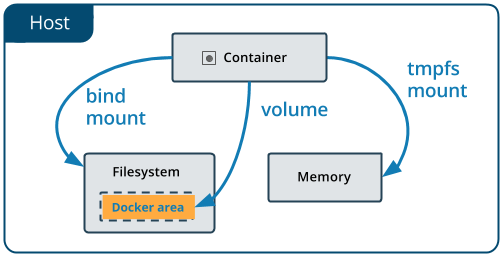
\includegraphics[width=.6\linewidth]{kapitel/problemloesung/implementierung/_img/types-of-mounts-volume}
	\caption[Docker Volumes -- Schaubild]{Docker Volumes -- Schaubild \cite[Kapitel~/storage/volumes/]{docker-doc}}
	\label{fig:dockerImage}
\end{figure}

Daten, die über Volumes persistiert werden, sind vom Betriebssystem des Hosts komplett unabhängig. Die Daten können dabei in dem \emph{writeable layer} des Containers selbst gespeichert werden\footnote{Erinnerung: Alle Schichten des Images werden als \emph{read-only} Systeme deployed, erst während der Initialisierungsphase des Containers wird eine weitere Schicht hinzugefügt, die während der Containerlaufzeit bearbeitet werden kann.}. Diese Daten werden allerdings verworfen, sobald der Container gelöscht wird. Um Daten auch weiterhin zu behalten und in neue Container-Instanzen laden zu können, wird hierbei auf Volumes zurückgegriffen. Es gibt zwei Varianten von Volumes \cite[Kapitel~/storage/volumes]{docker-doc}: 

\begin{enumerate}
  \item \emph{Named volumes}: have a specific source from outside the container, for example \verb+awesome:/bar+.
  \item \emph{Anonymous volumes}: have no specific source so when the container is deleted, instruct the Docker Engine daemon to remove them.
\end{enumerate}

Im Projekt wurde auf anonyme Volumes zurückgegriffen (siehe Listing \ref{lst:composeVolumes} \nameref{lst:composeVolumes}). Diese werden direkt vom Docker-Daemon verwaltet, wobei sich der Anwender damit nicht zu beschäftigen braucht. Neben den genannten Volume-Varianten gibt es ebenfalls die Möglichkeit, sogenannte \emph{bind mounts} zu verwenden. Diese sind jedoch abhängig von der Verzeichnisstruktur des Hosts sowie vom Betriebssystem, welches auf dem Host ausgeführt wird und gelten deshalb als veraltet. In der Dokumentation von Docker selbst wird empfohlen Volumes zu verwenden.

\paragraph{Docker Swarm}
Mit diesem Werkzeug ist es möglich, den definierten Komponentenstack in einer skalierten Umgebung darzustellen. Das Tool agiert als Orchestrator\footnote{Begriffserklärung siehe Abschnitt \ref{sec:anforderungPlattform} \nameref{sec:anforderungPlattform}.}. Die Container agieren hierbei im sogenannten "\emph{Swarm Mode}". Dabei können mehrere Maschinen derartig agieren, dass es für den Anwender den Anschein erweckt, als würde er lokal auf der eigenen Maschine arbeiten, wenn in Wirklichkeit ein ganzes Rechner-Netzwerk mit dem Hosten der Container betraut werden kann. Im Zusammenhang mit dieser Thesis ist allerdings das Skalieren einzelner Services der primäre Vorteil des Tools. Es ist möglich mehrere sogenannte \emph{Replicas} zu starten und auch wieder herunterzufahren, ohne dass die restlichen Stack-Komponenten hiervon beeinflusst werden. Um dies nutzen zu können, muss der definierte Stack von diesem Werkzeug übernommen werden. Zum gegenwärtigen Zeitpunkt bietet das Swarm-Werkzeug allerdings lediglich teilweise Unterstützung für das Einlesen der docker-compose Beschreibungsdatei. Vor allem wird das Setzen von Umgebungsvariablen mithilfe definierter Variablen des Buildsystems nicht unterstützt. In einer Produktivumgebung muss es jedoch die Möglichkeit geben, Umgebungsvariablen über Variablen des Buildsystems zu definieren; die Alternative wäre ansonsten auf \emph{hardcoded values} zurückzugreifen. Dies ist gerade hinsichtlich sensitiver Daten, zum Beispiel bei Anmeldedaten für Datenbanken etc., katastrophal. Um dennoch in der Lage zu sein, bestimmte Konfigurationsparameter mit Umgebungsvariablen füllen zu können, gibt es die Möglichkeit, das Docker-Compose-Werkzeug selbst als Präprozessor zu verwenden. Dabei wird das tool-konforme docker-compose Skript in ein Swarm-konformes Skript umgewandelt und die Umgebungsvariablen direkt mit den im System hinterlegten Werten ausgewechselt (siehe Schaubild \ref{fig:dockerComposeOverview} \nameref{fig:dockerComposeOverview}). Hierfür reicht ein entsprechender Aufruf über das CLI der Docker-Engine. Anschließend kann ein Swarm auf der Hostmaschine initialisiert und die Stack-Konfiguration deployed werden. In der Ausführung wird hierfür wieder auf ein Skript zurückgegriffen, was diese manuellen Shell-Befehle automatisiert\footnote{kompletter Dateiinhalt unter folgender Url einsehbar: \url{https://github.com/derMacon/serverless-bsc-thesis/blob/main/anhang/refs/start-stack-services.sh}}.

\begin{figure}[ht!]
	\centering
	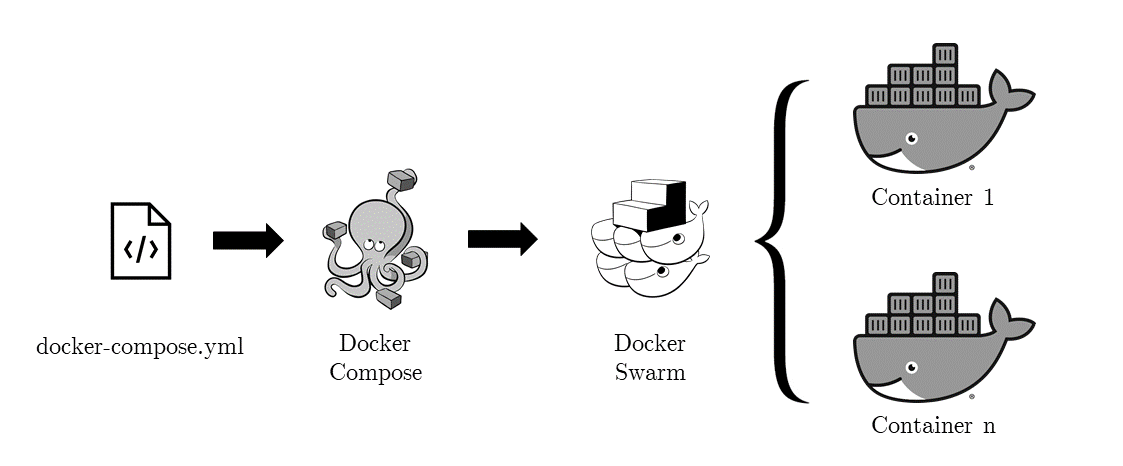
\includegraphics[width=.95\linewidth]{kapitel/problemloesung/implementierung/_img/stack-compose}
	\caption[Docker Compose -- Schaubild]{Docker Compose -- Schaubild}
	\label{fig:dockerComposeOverview}
\end{figure}

\begin{minipage}{\linewidth}
\begin{lstlisting}[style=bashStyle,caption={start-stack-services.sh},label=lst:summary-start-stack-services]

  ...

  echo 'use docker-compose as preprocessor for environmental variables'
  docker-compose -f $STACK_DIR/docker-compose.yml config > $STACK_DIR/docker-compose-parsed.yaml

  if [ ! isSwarmNode ]; then
    echo 'init swarm'
    docker swarm init
  fi

  echo 'redeploy stack'
  docker stack rm vossibility
  docker stack deploy --compose-file $STACK_DIR/docker-compose-parsed.yaml vossibility
\end{lstlisting}
\end{minipage}

Über den Befehl \verb+docker stack services vossibility+ lässt sich anschließend kontrollieren, ob der Stack gestartet ist und wie viele Serviceinstanzen jeder Komponente aktiv laufen. Die Ausgabe ist in Listing \ref{lst:supplierDockerfile} zu erkennen.

% \begin{landscape}
\begin{lstlisting}[style=javaStyle,caption={Dockerfile - Supplier},label=lst:supplierDockerfile]
  $ docker stack services vossibility
  ID             NAME                               MODE         REPLICAS   IMAGE                              PORTS
  mct16nrd6e91   vossibility_activemq               replicated   1/1        bwolf/activemq-prometheus:latest   *:8080->8080/tcp, *:8161->8161/tcp, *:61613->61613/tcp, *:61616->61616/tcp
  izrbys8vxive   vossibility_alertmanager           replicated   1/1        prom/alertmanager:v0.20.0          *:9093->9093/tcp
  jibw9j22qsrd   vossibility_consumer-db            replicated   1/1        postgres:13-alpine                 *:9292->9292/tcp
  rfocmjjuwzp8   vossibility_consumer-persistence   replicated   1/1        consumer-persistence:latest        *:8965->8965/tcp
  xu48nv8p1mvi   vossibility_grafana                replicated   1/1        grafana/grafana:latest             *:3000->3000/tcp
  orsxfojfj7u3   vossibility_history-db             replicated   1/1        postgres:13-alpine                 *:7004->7004/tcp
  yh3ykz5ixfaw   vossibility_node-consumer          replicated   1/1        node-consumer:latest
  ubeyrrzvatpq   vossibility_pgadmin                replicated   1/1        dpage/pgadmin4:latest              *:5050->5050/tcp
  7m4bpz6t166b   vossibility_prometheus             replicated   1/1        prom/prometheus:v2.21.0            *:9000->9090/tcp
  bfx1zqkg5oq0   vossibility_scaler                 replicated   1/1        thomasjpfan/docker-scaler:master   *:8743->8080/tcp
  32bd0chtwvjg   vossibility_scaler-proxy           replicated   1/1        scaler-proxy:latest                *:9245->9245/tcp
  twrq504kngog   vossibility_spring-consumer        replicated   1/1        spring-consumer:latest             *:7143->7143/tcp
  j57rwkmj7xr3   vossibility_supplier-backend       replicated   1/1        supplier-backend:latest            *:8284->8284/tcp
  f4wdecxpqxks   vossibility_supplier-frontend      replicated   1/1        supplier-frontend:latest           *:7384->80/tcp
\end{lstlisting}
% \end{landscape}

\section{Implementierung des Lasttests}
Nachdem im letzten Abschnitt auf die Konfiguration des Stacks eingegangen wurde, wird im Folgenden erklärt, welche Szenarien für die Messdatenerhebung durchgeführt wurden und unter welchen Bedingungen das System diese bearbeitet hat.

\subsection{Testszenarien}
Für die Erhebung der Messdaten wurde auf die in Abschnitt \ref{ss:Input} beschriebenen Skripte zurückgegriffen. Es wurde ein Aufruf des Skripts \emph{generate-traffic.sh} durchgeführt. Dieser sammelt im ausgeführten Verzeichnis rekursiv alle verfügbaren \emph{.benchmark} Dateien und schickt diese der Reihe nach über das \emph{curl-benchmark.sh} Skript an die Supplier-Schnittstelle. Die Skripte wurden dabei derartig organisiert, dass zu Beginn Skripte mit weniger Nachrichten in das System eingepflegt wurden, sodass es zu kleineren Skalierungssprüngen kam. Im späteren Verlauf wurde die Nachrichtenanzahl jedoch stetig erhöht, was wiederum in einem größeren Skalierungsaufkommen resultierte. Die folgende Abbildung (siehe Schaubild \ref{fig:benchmarkQueues} \nameref{fig:benchmarkQueues}) zeigt die Daten des Message Brokers. 

\begin{figure}[ht!]
	\centering
	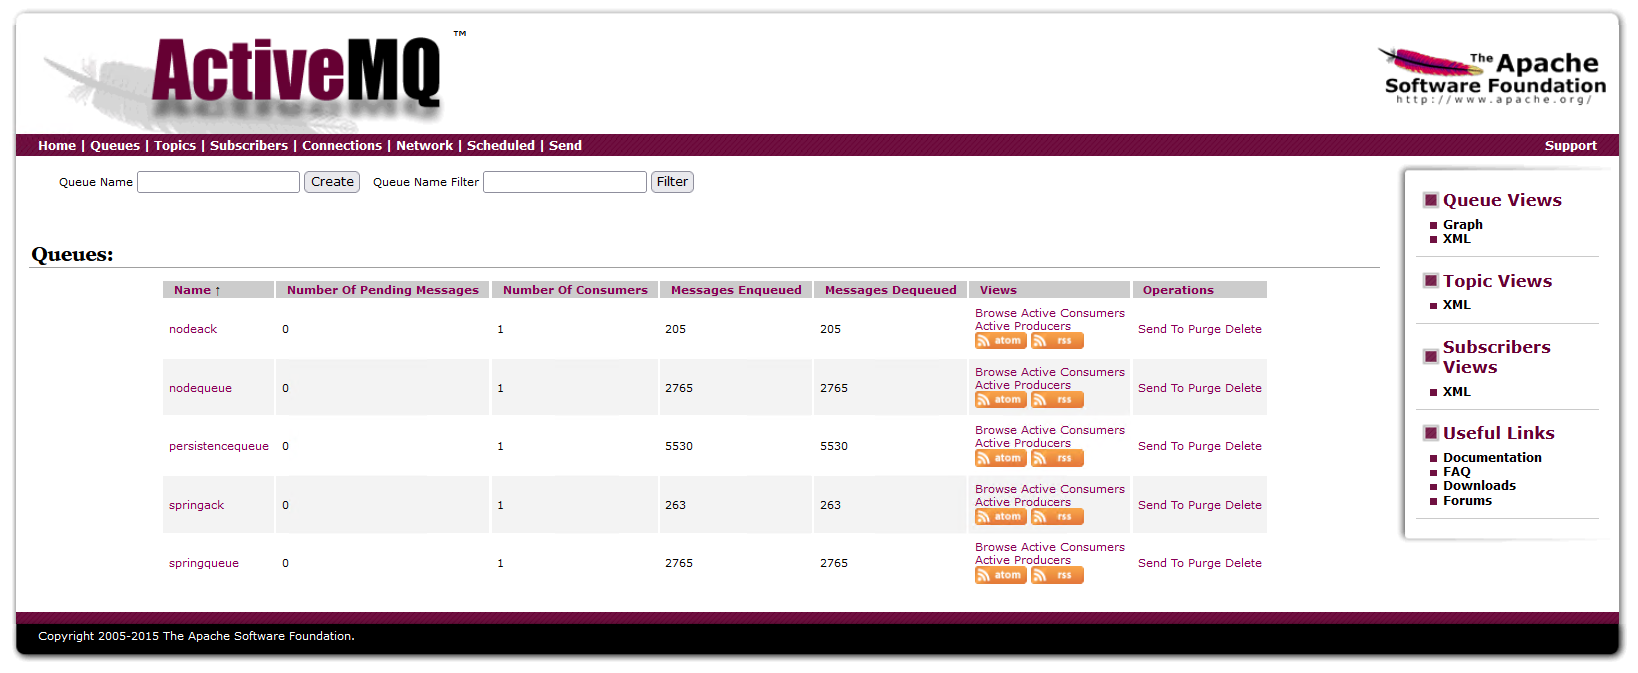
\includegraphics[width=\linewidth]{kapitel/problemloesung/implementierung/_img/benchmark-queues}
	\caption[Benchmark - Queues]{Benchmark - Queues}
	\label{fig:benchmarkQueues}
\end{figure}

Es wurden für dieses Testszenario insgesamt 5530 Nachrichten verschickt und bearbeitet. Dies ist daran zu erkennen, dass die \emph{persistencequeue} entsprechend viele Einträge verwaltet hat. Die Hälfte wurde jeweils von der Node.js- sowie Spring-Boot-Komponente bearbeitet (siehe \emph{nodequeue} sowie \emph{springqueue}). In der Praxis muss ein System allerdings eine deutlich höhere Last verarbeiten können. Das Produktivsystem des Unternehmens ist in der Lage, 1000 Nachrichten pro Sekunde verarbeiten zu können. In entsprechenden Lasttests wird dies über einen Zeitraum von einer Stunde oder mehr getestet. Für diesen Prototypen ist die genannte Anzahl allerdings völlig ausreichend, um einen Überblick über das System zu bekommen. Außerdem wurde in den verarbeitenden Komponenten vom Prototypen eine künstliche Verlangsamung in Form eines Sleep-Aufrufs am Ende des Arbeitsflusses hinzugefügt, um eine bessere Nachvollziehbarkeit zu gewährleisten, welche in der Produktivumgebung natürlich entfällt.

Der primäre Unterschied der beiden Services zeigt sich jedoch in der hochgefahrenen Containeranzahl. Um dem System mitzuteilen, dass ein neuer Container erfolgreich hochgefahren ist, setzt dieser eine Nachricht in die \emph{nodeack} beziehungsweise die \emph{springack} Warteschlange ab. Wie zu erkennen ist, wurden insgesamt 205 Node.js-Container und 263 Spring Boot Container über den gesamten Zeitraum des Testszenarios hochgefahren. Dieser Unterschied lässt sich mit der unterschiedlich langen Initialisierungsphase der Komponenten begründen (mehr dazu Abschnitt \ref{ss:skalierungsdauer} \nameref{ss:skalierungsdauer}).

Das zweite Testszenario betrifft die direkte Skalierung mithilfe des Skripts \emph{direct-scaling.sh}. Hierbei wird die Proxy-Scaler Komponente direkt angesprochen (Erklärung siehe Abschnitt \ref{ss:bash} \nameref{ss:bash}). Der Aufruf wurde mit einem \emph{Offset} Parameter von 29 und einer Wiederholungsanzahl von 10 getätigt. Insgesamt wurden für dieses Testszenario demnach 290 Skalierungsanfragen pro Service an die Proxy-Komponente geleitet. Beide Services wurden hierbei 4350 Mal neu hochgefahren\footnote{Summe 1 bis 29 = 435, jeder Skalierungsschritt wurde 10 Mal wiederholt: 435 * 10 = 4350}.

\subsection{Testbedingungen}
% \begin{itemize}
%   \item Kommt in den Anhang
%   \item hat Prof. zwar als eigenes Kapitel erwaehnt, bin mir aber nicht sicher ob das wirklich noetig ist
%   \item auf welcher Hardware werden Tests durchgefuehrt?
%   \item chaos monkey / Stoerfaelle erlaeutern
% \end{itemize}

Sämtliche erhobenen Daten werden auf einem System getestet, wie es in der folgenden Tabelle beschrieben wird. 

\renewcommand\theadalign{bc}
\renewcommand\theadfont{\bfseries}
\renewcommand\theadgape{\Gape[4pt]}
\renewcommand\cellgape{\Gape[4pt]}

\begin{table}[ht!]
  \centering
  \bigskip
  \begin{tabular}{ c l }
    \toprule
    Prozessor & Intel(R) Xeon(R) Gold 6226R CPU @ 2.90GHz \\
    \midrule
    Kerne & 6 Prozessoren á 16 Kerne \\
    \midrule
    RAM & 16 GB \\
    \midrule
    Storage & 150 GB \\
    \midrule
    Distro & CentOS 8\\
    \bottomrule
  \end{tabular}
  \caption{Server Specs}
  \label{tab:serverSpecs}
\end{table}


\subsection{Zusammenfassung}
Da sich dieser Abschnitt in erster Linie auf die Implementierung der einzelnen Komponenten konzentriert, wird im Folgenden auf eine detailliertere Zusammenfassung verzichtet. 
